%
% Grizzards printable manual
%
% This needs a lot of work yet.
%
% If you're a human, skip to "\mainmatter" to skip over the preamble.
%
\documentclass[9pt,twocolumn,openany,article,crop]{memoir}
\ifdefined\ATARIAGESAVE
\setstocksize{7.25in}{5.25in}
\setpagecc{7in}{5in}{*}
%\setlength\normalsize
\else
\setstocksize{11in}{8.5in}
\settrimmedsize{\stockheight}{\dimexpr 8.5in-15mm}{*}
\fi

\setlrmarginsandblock{.4in}{.5in}{*}
\setulmarginsandblock{.6667in}{.6667in}{*}
\setheadfoot{.45in}{.45in}
\widowpenalty=10000
\clubpenalty=10000
\raggedbottom

\makeevenhead{plain}{\textit{Grizzards}}{}{}
\makeoddhead{plain}{}{}{\textit{Grizzards}}

\makeevenfoot{plain}{\thepage}{}{}
\makeoddfoot{plain}{}{}{\thepage}

\usepackage[utf8]{inputenc}
\usepackage{babel}
\usepackage{stfloats}
\usepackage{microtype}
\usepackage{graphicx}
\usepackage{pdfpages}
\tolerance=1
\emergencystretch=\maxdimen
%\usepackage{tgtermes}
\usepackage{hyperref}
\usepackage{xcolor}
\hypersetup{
    colorlinks,
    linkcolor={black},
    citecolor={blue!50!black},
    urlcolor={blue!80!black},
    pdftitle={Grizzards \ifdefined\DEMO{ Demo }\fi{}Manual},
    pdfsubject={Grizzards videogame for the Atari 2600},
    pdfauthor={Bruce-Robert Pocock}%,
%    pdfkeywords={Your PDF keywords}
  }
\usepackage{caption}
\captionsetup{labelformat=empty}
\usepackage{fontspec}
\setmonofont{Source Code Pro}

\usepackage{tikz}

\newcommand\encircle[1]{%
  \tikz[baseline=(0,3pt)]
  \draw (0,0) circle [radius=5.25pt] node {{\footnotesize\textbf{#1}}};}

\newenvironment{ritemize}{\begin{itemize}\raggedright}{\end{itemize}}
\newenvironment{rdescribe}{\begin{description}\raggedright}{\end{description}}

\newcommand\picaskip{\vspace{12pt}}
\newcommand\englishskip{\vspace{14pt}}

\setlength{\columnsep}{.333333in}
% \setlength\columnseprule{.5pt}

\usepackage{lettrine}
\usepackage[protrusion=true,expansion=true]{microtype}
\fontfamily{bch}
\chapterstyle{komalike}

\checkandfixthelayout

\title{Grizzards \ifdefined\NOSAVE No-Save \fi\ifdefined\DEMO Demo \fi Player's Guide}
\author{Bruce-Robert Pocock}

%
%
%
%%% BEGIN DOCUMENT
%
%
%

\begin{document}

\frontmatter
\thispagestyle{empty}\noindent
\ifdefined\ATARIAGESAVE
\begin{tikzpicture}[overlay, remember picture]
  \node[anchor=north west, xshift=-3.25pt, yshift=21.25pt] 
  at (current page.north west)
  {\noindent{}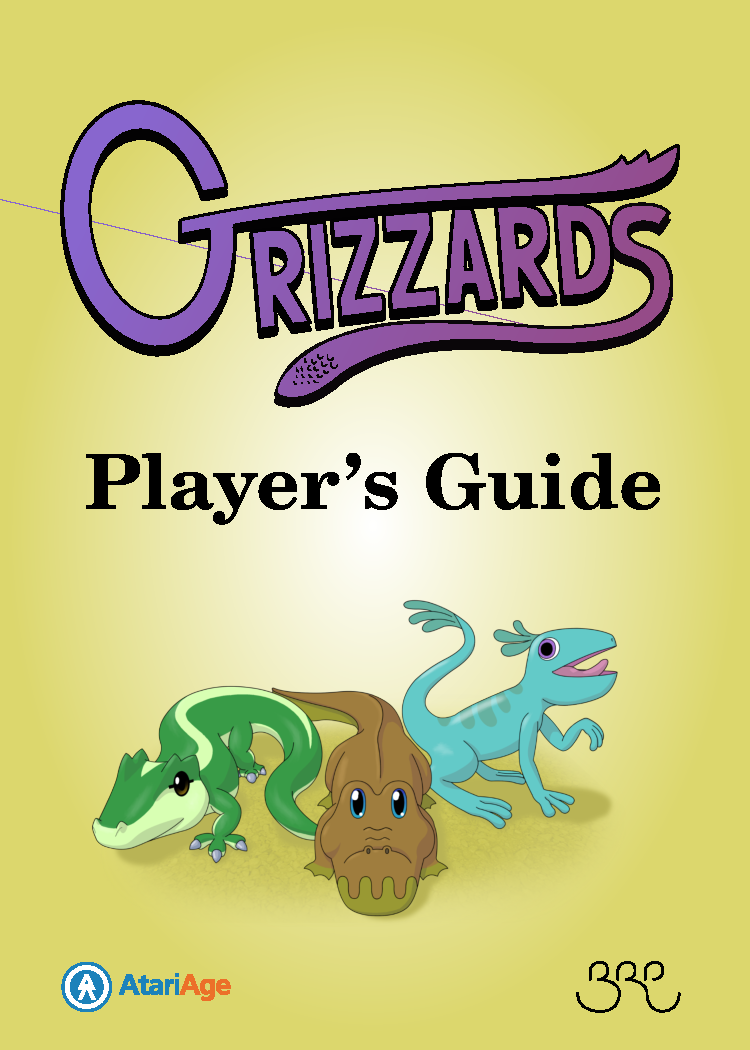
\includegraphics[width=5.25in,height=7.25in,interpolate]{../Manual/Cover.pdf}};
\end{tikzpicture}
\else
\begin{tikzpicture}[overlay, remember picture]
  \node[anchor=north west, xshift=-4pt, yshift=4pt] 
  at (current page.north west)
  {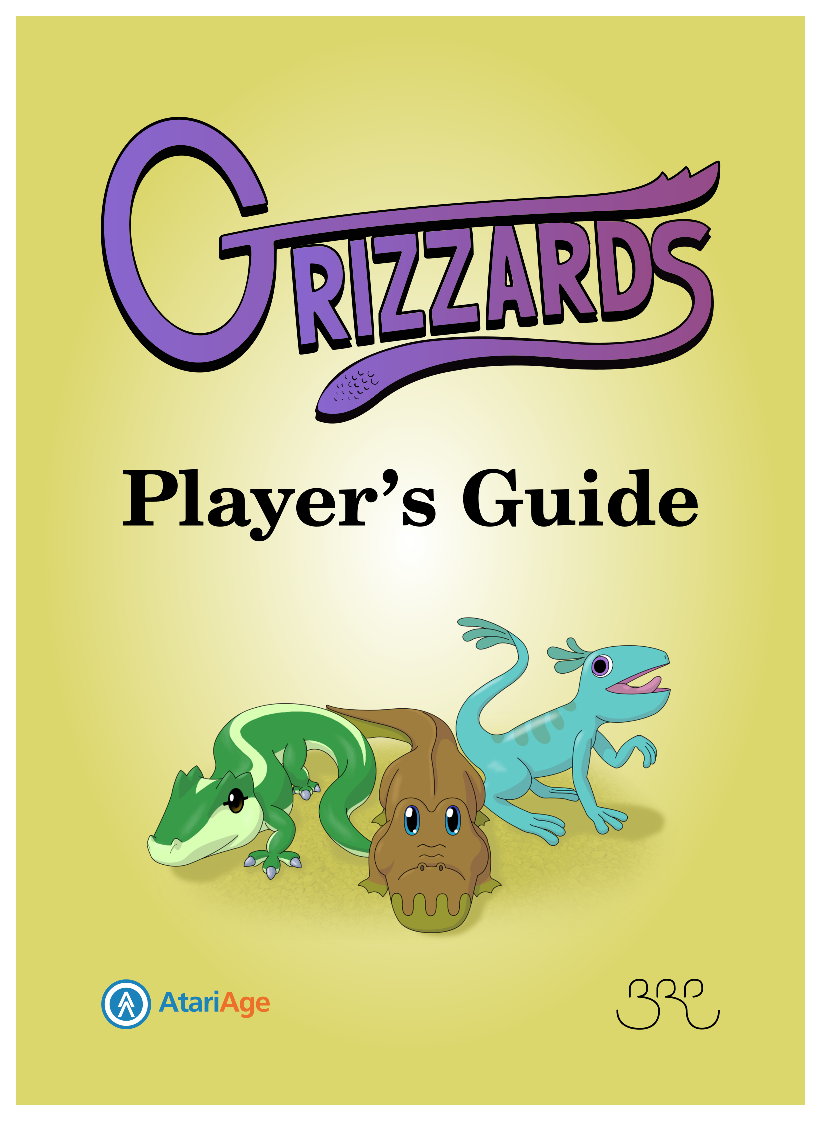
\includegraphics[width=\paperwidth,height=\paperheight]{../Manual/Cover.eps}};
\end{tikzpicture}
\fi

\thispagestyle{empty}

\twocolumn[

\chapter*{Introduction}\label{Introduction}

The  land of  Syrex  is  a dangerous  place.  Fierce  monsters roam  the
countryside. But luckily for you, you're a Grizzard handler!

\bigskip

Train your Grizzard to  use a variety of Moves to  take on the monsters.
Discover new kinds  of Grizzards with new capabilities.  Can you conquer
all the monsters of Syrex?

\bigskip

In the  \textit{Grizzards} videogame, you'll  roam the land  looking for
monsters. Monsters may  surprise you as you travel, or  you may see them
coming. When faced  with terrifying beasts, you'll  direct your Grizzard
to use its Moves to defend you and attack the monsters.

\vfill
\noindent\rule{\pagewidth}{0.4pt}
\picaskip

{ \footnotesize This is the \textit{Grizzards} \ifdefined\NOSAVE No-Save
  \fi\ifdefined\DEMO  Demo   \fi\ifdefined\ATARIAGESAVE  Official  \else
  Public Release \fi Player's Guide. }

\picaskip

{ \footnotesize The \textit{Grizzards} videogame software, including its
  audiovisual  components and  this manual,  are copyright  \copyright{}
  2022, Bruce-Robert Pocock.  All Rights are Reserved  except as granted
  under license. }

\picaskip

{ \footnotesize For Atari Video  Computer System CX-2600 (or compatible)
  \ifdefined\ATARIAGESAVE   with   optional   AtariVox   device.   \else
  \ifdefined\NOSAVE  without \else  with  \fi AtariVox  (or MemCard,  or
  SaveKey)  device. \fi  Screenshots represent  the NTSC  version; other
  versions have distinct coloring. }

\picaskip

{ \footnotesize This  videogame software was not  created, published, or
  licensed by Atari or its successors. }

\picaskip

\ifdefined\DEMO
\bigskip

This manual  describes a \ifdefined\NOSAVE  No-Save \fi DEMO  version of
the game. The full version may be different.

\fi

Published by AtariAge. \href{https://atariage.com/}{https://atariage.com/}

\ifdefined\ATARIAGESAVE\else  If you  enjoy playing  \textif{Grizzards},
you  may  be  interested  in  purchasing a  retail  copy  with  built-in
save-game    memory    from    AtariAge.    Coming    in    2022.  
\href{https://atariage.com/}{https://atariage.com/}

\bigskip

You are hereby granted permission  to make use of the \textit{Grizzards}
videogame software for \emph{non-commercial personal use}.

Redistribution not for profit is allowed, but sales of this software
requires a license.

\fi

\picaskip]

\begin{center}
  
\includegraphics[width=1.5in]{../Manual/AtariVoxEnhanced.eps}
\end{center}

\let\cleardoublepage\clearpage

\mainmatter

\tableofcontents

\twocolumn[\chapter{Setting Up}\label{Setting Up}]

\noindent{}To play \textit{Grizzards}, you will need:

\picaskip

\begin{ritemize}
\item  An Atari  console: the  Atari  Video Computer  System CX-2600  or
  a compatible console
\item A TV or video display
\item A joystick controller or a compatible gamepad
  \ifdefined\ATARIAGESAVE
  \item Optional: an AtariVox device with speakers or headphones
  \else
  \ifdefined\NOSAVE\else
\item A  memory device: an  AtariVox device with (optional)  speakers or
  headphones, or a MemCard or SaveKey device.
  \fi\fi
\item The \textit{Grizzards} game cartridge \ifdefined\ATARIAGESAVE\else
  or a multi-cart with the \textit{Grizzards} data on it. \fi
\end{ritemize}

\ifdefined\ATARIAGESAVE\else
\ifdefined\NOSAVE\else
\begin{figure*}[b]
  \begin{center}
    \ifdefined\ATARIAGESAVE
    \includegraphics[width=\columnwidth]{../Manual/Atari-2600-Wood-4Sw-Set.png}
    \else
    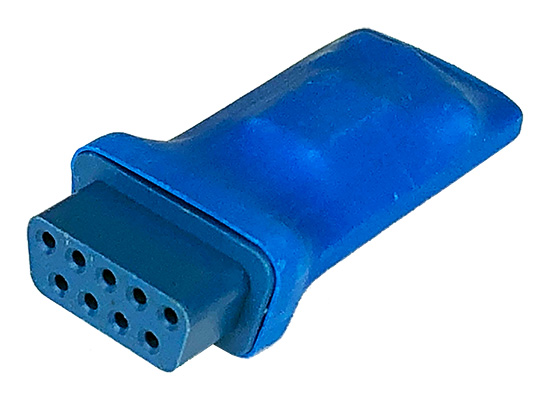
\includegraphics[width=\columnwidth]{../Manual/SaveKey.jpeg}
    \fi
    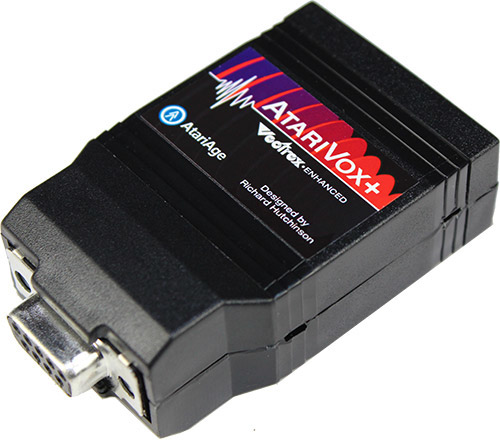
\includegraphics[width=.75\columnwidth]{../Manual/AtariVox.jpeg}
  \end{center}
\end{figure*}
\fi
\fi

Set up  your console with your  TV or video display.  Connect a joystick
(or gamepad) to  the \emph{left} controller port\ifdefined\ATARIAGESAVE,
and  (optionally) your  AtariVox device  to the  \emph{right} controller
port.  \else\ifdefined\NOSAVE.\else{},  and  the memory  device  to  the
\emph{right} controller port.

The  retail  cartridge (available  later  in  2022 from  AtariAge)  will
\emph{not}  require  a  memory   device  because  the  special  AtariAge
cartridge contains its own save-game memory within it.

To purchase \textit{Grizzards}, SaveKey,  AtariVox+, or many other Atari
games,                                                             visit
\href{https://atariage.com/store/}{https://AtariAge.com/store/}

\fi\fi

Finally, insert  the \textit{Grizzards}  game cartridge (with  the label
facing  up)  into  the  cartridge  slot,  and  turn  the  \textbf{Power}
\textbf{on}.

% \ifdefined\ATARIAGESAVE
% \vfill
% \fi

\includegraphics[width=.8\columnwidth]{../Manual/Atari-2600-Wood-4Sw-Set.png}

\pagebreak

\section{Using a Gamepad}\label{sec:Gamepad}

  A  SEGA  Genesis/MegaDrive   gamepad  (or  other
compatible controller) may also be  used. Use the \encircle{B} button as
the \textbf{Fire} button. Use the  \encircle{C} button as an alternative
way  to   press  the   \textbf{Game  Select}   switch  to   access  your
Grizzard's statistics.

A ``Joy2b$^+$'' game pad, such as those from 
\href{https://retrogameboyz.com/products/atari-8-bit-2-button-action-joystick-control-pad-gamepad-xegs-theme?variant=39665422565431}{RetroGameBoyz.com},
can also  be used.  Button \encircle{I} will  work as  the \textbf{Fire}
button.  Button  \encircle{II} will  work  as  the \textbf{Game  Select}
switch. Button \encircle{III} will toggle pausing the game.

An    Atari     7800    controller     will    \emph{not}     work    as
a two-button controller, even on an Atari 7800 console.

Your gamepad  \emph{must} be  plugged in \emph{before}  you turn  on the
power, or the extra  buttons will not work. \ifdefined\ATARIAGESAVE\else
If using a \ifdefined\DEMO Harmony or \fi Harmony Encore cartridge, hold
down  the \encircle{B}  or \encircle{I}  button when  you power  on your
console, or the gamepad will not work on the Harmony menu. \fi

\ifdefined\ATARIAGESAVE
\vfill
\begin{center}
  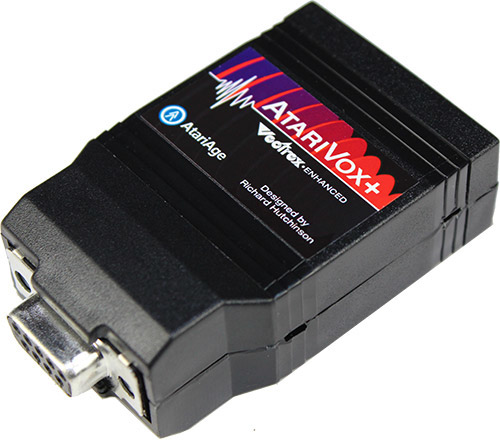
\includegraphics[width=.6667\columnwidth]{../Manual/AtariVox.jpeg}
\end{center}
\fi

\pagebreak
\twocolumn[\chapter{How To Play}]

\section{Console Controls}

\subsection{Pausing the Game}

On an Atari 2600  (or similar console), with the NTSC  or PAL version of
the game,  push the  \textbf{Color/B\&W} switch into  the \textbf{Color}
position  to play  the game,  or  the \textbf{B\&W}  position to  pause.

With the SECAM  version of the game, the Right  Difficulty Switch can be
used  to  pause game  play.  When  in  the  ``A'' (Advanced  or  Expert)
position, your  game will be paused.

On the  Atari 7800, press  the \textbf{Pause}  button once to  pause the
game, and again to resume playing. \ifdefined\ATARIAGESAVE\else This may
not work with certain multi-carts, e.g. the UnoCart or PlusCart. \fi

\subsection{Game Select}

When viewing  the Title Screen,  use the \textbf{Game Select}  switch to
\ifdefined\NOSAVE begin your game or start  over \else choose a Slot and
begin or resume a game. \fi

While you  are playing the  game, use the  \textbf{Game Select}
switch to view your Grizzard's  statistics.

\subsection{Game Reset}

When  viewing the  Select  Slot screen,  press  the \textbf{Game  Reset}
switch to begin playing the game.

While you are playing the game,  press the \textbf{Game Reset} switch to
\emph{immediately} abandon your progress and return to the Title Screen.
You will  lose some  of your  progress since the  last time  you visited
a Grizzard Depot.

\ifdefined\NOSAVE\else

\subsection{Protecting Your Game Record}

You  cannot erase  a  game  in progress  (or  un-erase  it) unless  both
Difficulty  Switches are  in the  ``A'' (Advanced  or Expert)  position.
To protect your game from being erased, set either one of the Difficulty
Switches to the ``B'' (Beginner or Novice) position.

\fi

\subsubsection*{Expert Mode}

The Left Difficulty Switch adjusts the  difficulty of the game. When the
Left Difficulty  Switch is in  the ``A'' (Advanced or  Expert) position,
monsters will do more damage in their attacks. You will also earn double
points for defeating monsters while in the ``A'' position.

On the Atari 7800, the  Difficulty Switches (located near the controller
ports) are in the ``A'' position when they are moved to the right.

%%\ifdefined\ATARIAGESAVE\vfill\pagebreak\fi

\section{Starting a Game}

\begin{center}
  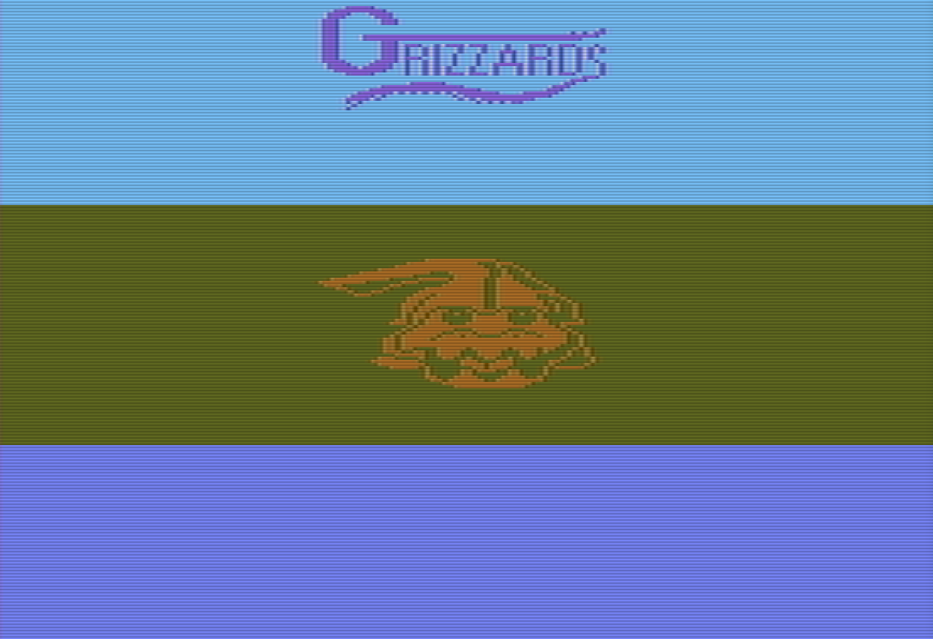
\includegraphics[width=.75\columnwidth]{../Manual/TitleAquaxNTSC.png}
\end{center}

Once your  console is set  up and everything  is connected, turn  on the
\textbf{Power} switch. You'll  see the title screen appear.  If you have
an AtariVox device, you'll also hear the title spoken.

Press the \textbf{Game Select} switch or \textbf{Fire} button to move to
the
\ifdefined\NOSAVE
Begin/Resume screen.

Press the  joystick left or  right to choose whether  to \texttt{RESUME}
your current game  in progress or \texttt{BEGIN} a new  game, then press
\textbf{Game Reset} or the \textbf{Fire} button.

\else
Select Slot screen.

\begin{center}
  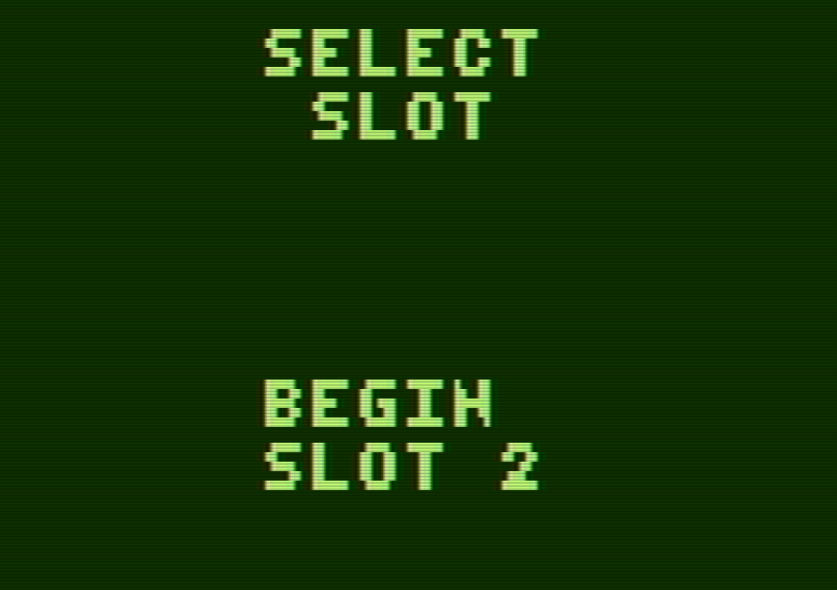
\includegraphics[width=.75\columnwidth]{../Manual/SelectSlotNTSC.png}
\end{center}

Press  the \textbf{Game  Select} switch  or move  the joystick  left and
right to  choose a  memory slot\ifdefined\ATARIAGESAVE\else\footnote{The
  Slot number chosen here is relative  to the three save game slots used
  by the \textit{Grizzards}  game program. Each save  game slot actually
  occupies  4  blocks  on  your  memory  device.}\fi{}  for  your  game.
There  are \ifdefined\ATARIAGESAVE  eight \else  three \fi  memory slots
available.

If someone  has already  begun to play  \textit{Grizzards} in  a certain
slot, your screen will show  \texttt{RESUME}, and their name will appear
as well. If a slot is empty, you'll see \texttt{BEGIN} instead.

If someone has already \emph{won} the  game once, their name will appear
in bright yellow. See ``New Game Plus,'' page~\pageref{sec:NewGamePlus}.

\ifdefined\DEMO

\skip

Your save game progress from the demo is \emph{not} transferable to the
full game.

\skip

\fi

When you have selected the slot in which to begin (or resume), press the
\textbf{Fire} button.

\fi

\ifdefined\NOSAVE\else

When you begin a  new game, enter your name. Push  forward to select the
next letter;  pull back to  select the  previous letter. Press  left and
right to move to  the previous or next position. You can  use up to six
characters for  your name.  After six characters,  the cursor  will turn
pink; then, press the \textbf{Fire} button to proceed.

\begin{center}
  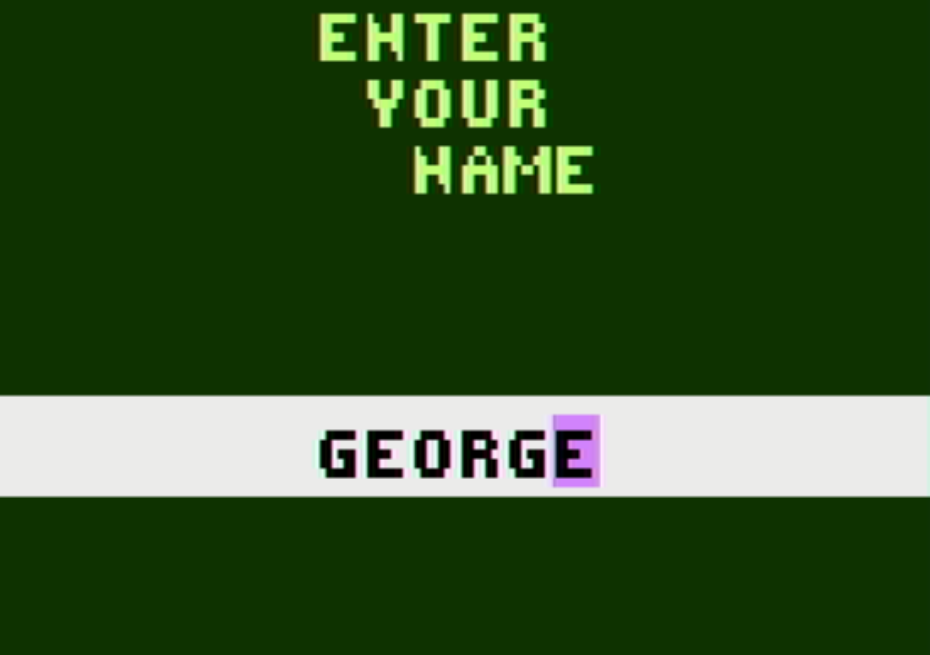
\includegraphics[width=.75\columnwidth]{../Manual/NameEntryNTSC.png}
\end{center}

\ifdefined\DEMO

In this demo,  you'll always begin with Aquax as  your companion. In the
full game, you can choose from one of three starting Grizzard companions.

\else

Next, you'll pick your starting Grizzard. There are three Grizzards from
which    to    choose:   Dirtex,    Aquax,    or    Airex.   Refer    to
Chapter~\ref{ch:Grizzards}   on  page~\pageref{ch:Grizzards}   for  more
information about each of them.

\begin{center}
  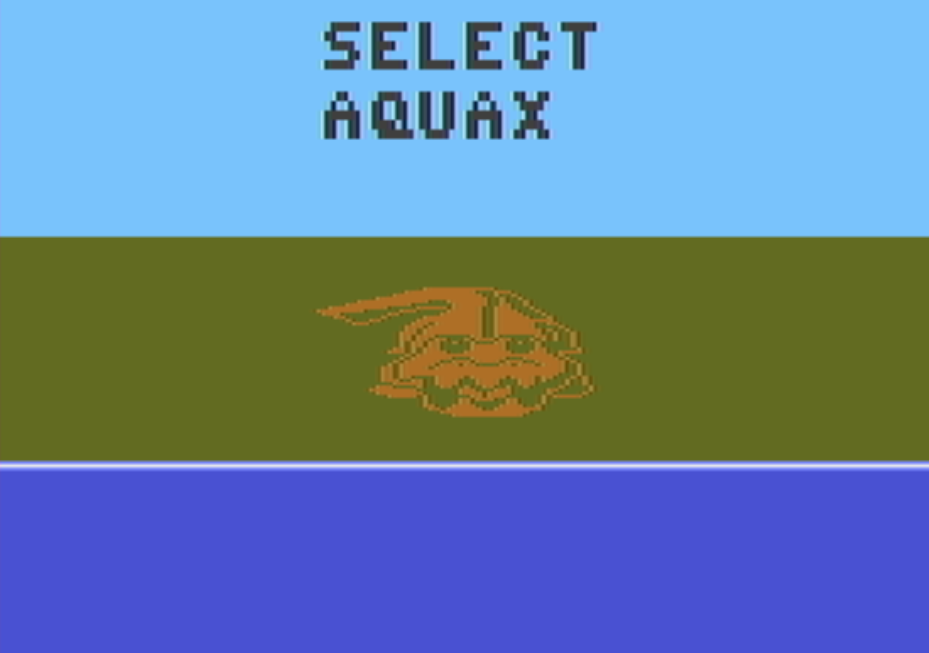
\includegraphics[width=.75\columnwidth]{../Manual/GrizzardChooserNTSC.png}
\end{center}

Press left  and right  to choose  a Grizzard  companion, then  press the
\textbf{Fire} button.

Make  sure  that you've  entered  your  name  correctly and  chosen  the
Grizzard companion  you prefer. Push  forward on the joystick  to select
\texttt{CHANGE} and edit your name and companion choice, or pull back to
choose    to   \texttt{BEGIN}    your   adventure    now.   Press    the
\textbf{Fire} button.

\begin{center}
  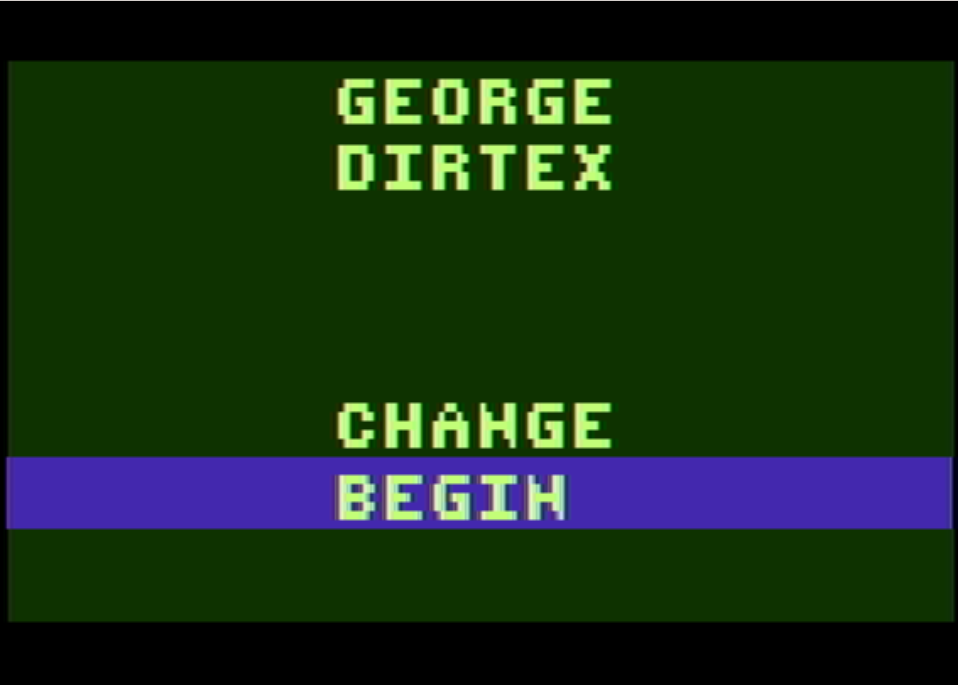
\includegraphics[width=.75\columnwidth]{../Manual/ConfirmNewGameNTSC.png}
\end{center}

\fi
\fi
\ifdefined\NOSAVE

In this no-save demo, you can only  play with one Grizzard at a time ---
starting with Aquax. The demo using  a memory device allows you to catch
other Grizzards. In the full game,  you can choose one of three starting
Grizzard companions.

\fi

\section{Exploring Syrex}

You'll begin in the ruins of  Treble Village after the monsters invaded.
You know that to  the east is the extremely dangerous  Fire Bog, so your
best  bet   is  to  head   west  (left)  and   see  if  there   are  any
other survivors.

The Map screen shows your current score  at the top. In the map display,
you'll see the  current area in which you are  traveling. Guide yourself
using the joystick.

\begin{center}
  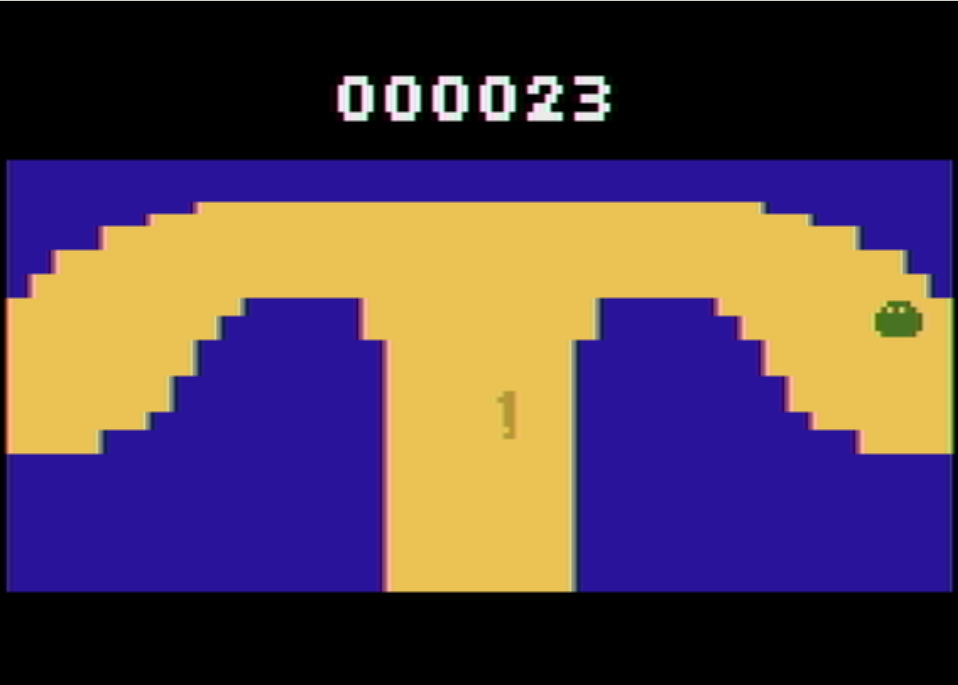
\includegraphics[width=.75\columnwidth]{../Manual/MapNTSC.png}
\end{center}

Refer to \ifdefined\ATARIAGESAVE  the included map \else the  map on the
last page  of this  manual \fi  to learn about  the geography  of Syrex.
Characters in the game will also give you advice.

You can check your inventory of potions,  and choose to give one to your
current  Grizzard  companion  by   pressing  the  \textbf{Fire}  button.
\ifdefined\DEMO However, there are no potions in this demo. \fi

To interact with something on the Map screen, just walk into it.

\englishskip

\lettrine[image=true,                lines=4,               findent=3pt,
nindent=3pt]{../Manual/MonsterNTSC.png}\nobreak\hspace{.2em plus 0}A     monster,    or
a group of monsters, may sneak up  on you and attack! Other times you'll
see them waiting for you and can  avoid battle --- or approach them when
you're ready to face them. Particularly giant monsters look different on
the map; you'll discover them in your travels.

\ifdefined\ATARIAGESAVE \pagebreak \else \englishskip \fi

\lettrine[image=true,                lines=4,               findent=3pt,
nindent=3pt]{../Manual/DepotNTSC.png}\nobreak\hspace{.2em plus 0}Grizzard~Depots~are
safe~spaces.~Your Grizzards will be healed\ifdefined\NOSAVE{}.{}\else{},
and your  progress will  be saved  \ifdefined\ATARIAGESAVE to  your game
cartridge. \else  to your memory device.  \fi You can also  switch which
Grizzard    is     your    current     companion.    \fi     See    page
\pageref{sec:GrizzardDepot} for details.

\englishskip

\ifdefined\NOSAVE

\lettrine[image=true,                lines=4,               findent=3pt,
nindent=3pt]{../Manual/WildGrizzardNTSC.png}\nobreak\hspace{.2em plus 0}Wild  Grizzards
roam  the land  sometimes.  In  this no-save  demo,  you  will have  one
Grizzard companion at a time, beginning with Aquax.

\else

\lettrine[image=true,                lines=4,               findent=3pt,
nindent=3pt]{../Manual/WildGrizzardNTSC.png}\nobreak\hspace{.2em plus 0}Wild  Grizzards
roam the  land sometimes. You  can catch  them when you  encounter them.
At  a   Grizzard  Depot,  you   can  change  your   Grizzard  companion.
Each  Grizzard  you  catch  will  have its  own  Moves,  skill  ratings,
and experience.

\fi

\englishskip

\lettrine[image=true,                lines=4,               findent=3pt,
nindent=3pt]{../Manual/DoorNTSC.png}\nobreak\hspace{.2em plus 0}Doors~can~lead~ you
to~other~places~in the world. \\

\englishskip

\lettrine[image=true,                lines=4,               findent=3pt,
nindent=3pt]{../Manual/SignpostNTSC.png}\nobreak\hspace{.2em plus 0}Signposts~provide
information~to~help   you   progress.   You   should   also   refer   to
\ifdefined\ATARIAGESAVE the included map. \else the map on the last page
of this manual. \fi

\englishskip

\lettrine[image=true,                lines=4,               findent=3pt,
nindent=3pt]{../Manual/PersonNTSC.png}\nobreak\hspace{.2em plus 0}People
will converse with you and can help you out. Some people will respond to
you differently based on what has come  before, so you may want to visit
them more than once.


\ifdefined\NOSAVE\else

\section{Saving Your Progress}

Your progress  is saved whenever  you visit  a Grizzard Depot.  Once you
hear the short musical tune, it is safe to power off your console.

\ifdefined\ATARIAGESAVE\else

You must leave  your memory device connected at all  times while playing
the game. Sometimes, the game may auto-save some of your progress.

\fi \fi

\section{Conversations}

When  you encounter  a person,  they'll  speak to  you. If  you have  an
AtariVox  connected,  you'll  hear  what  they have  to  say  out  loud.
After you've read it, press the \textbf{Fire} button.

\begin{center}
  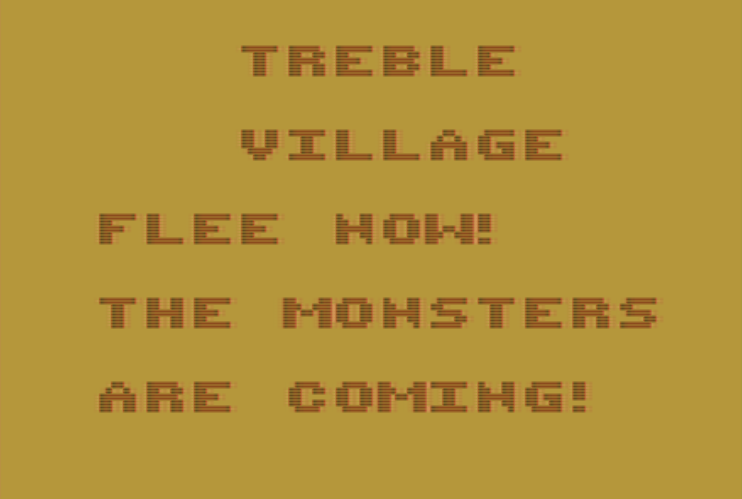
\includegraphics[width=.75\columnwidth]{../Manual/TextNTSC.png}
\end{center}

Some people will want you to answer a question. You'll be given a choice
of two possible answers. Push forward and back on the joystick to select
a response.

\begin{center}
  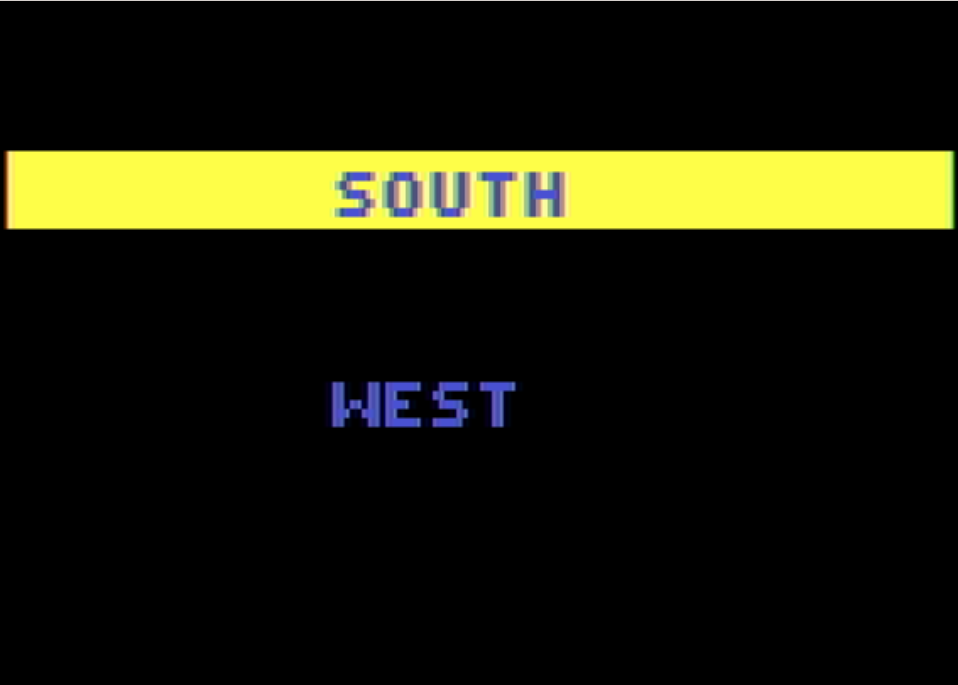
\includegraphics[width=.75\columnwidth]{../Manual/InquireNTSC.png}
\end{center}

To review  what  the  person  was  asking, press  left  on
the joystick.

When you've made your selection, press the \textbf{Fire} button to continue.

%% \ifdefined\ATARIAGESAVE
%% \pagebreak
%% \fi
\begin{figure*}[t]
  \begin{center}
    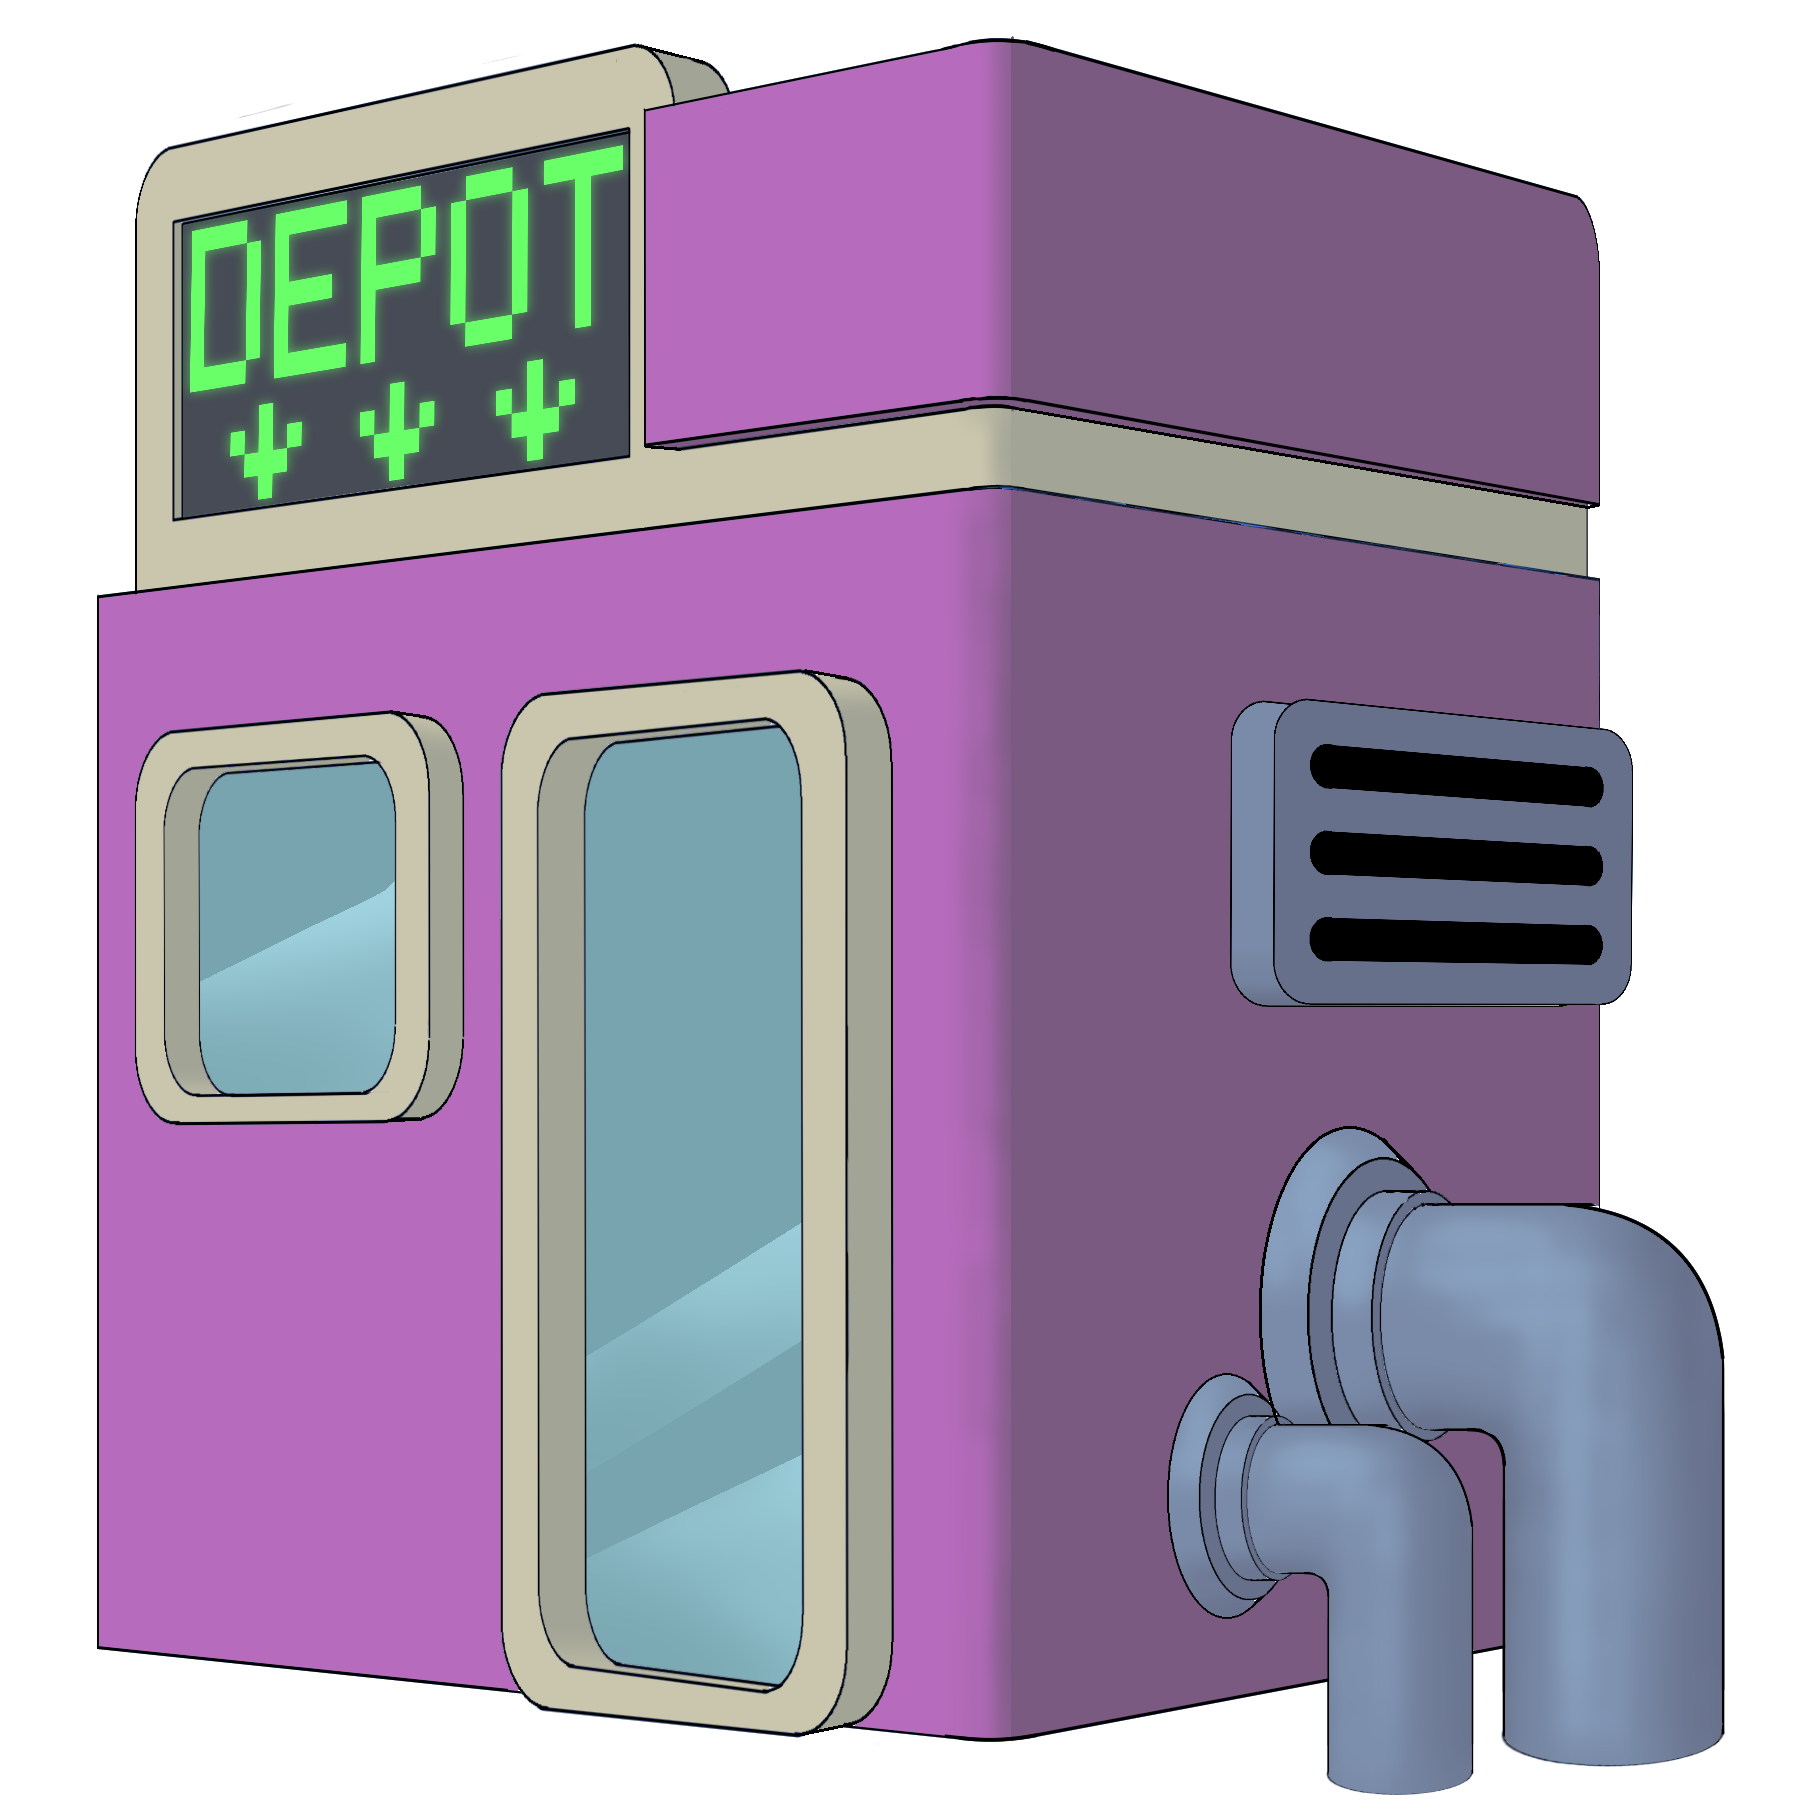
\includegraphics[width=1.6667\columnwidth]{../Manual/GrizzardDepot.png}
  \end{center}
\end{figure*}

\section{Grizzard Depots}\label{sec:GrizzardDepot}

To  \ifdefined\NOSAVE\else swap  or  \fi heal  your Grizzard  companion,
you'll need to visit a Grizzard Depot.

\begin{center}
  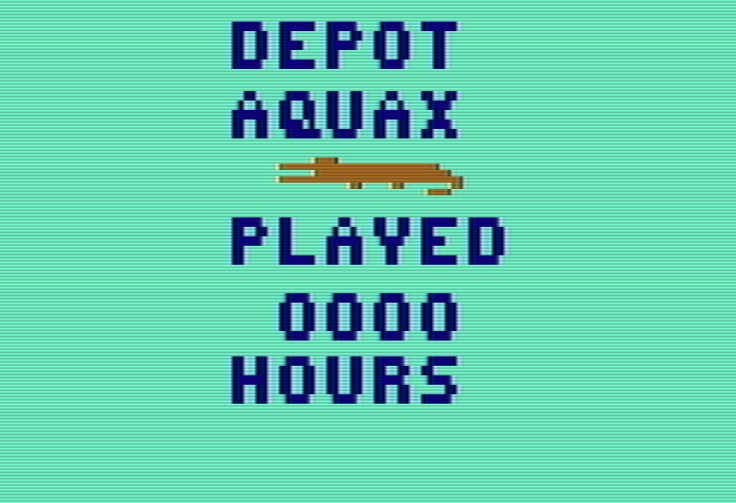
\includegraphics[width=.75\columnwidth]{../Manual/DepotScreenshotNTSC.png}
\end{center}

\ifdefined\NOSAVE\else Your progress will \emph{immediately} be saved to
your \ifdefined\ATARIAGESAVE  game cartridge,  \else memory  device, \fi
\fi   and    your   Grizzard    companion   will   be    fully   healed.
\ifdefined\NOSAVE\else  Push the  joystick  forward and  back to  choose
a different Grizzard to travel with you. \fi

To  view  your Grizzard's  statistics,  press  the \textbf{Game  Select}
switch or move  the joystick left or right. When  you're ready to return
to your adventure, press the \textbf{Fire} button.

\section{Battling Monsters}

% \begin{figure*}[t]
%   \begin{center}
%     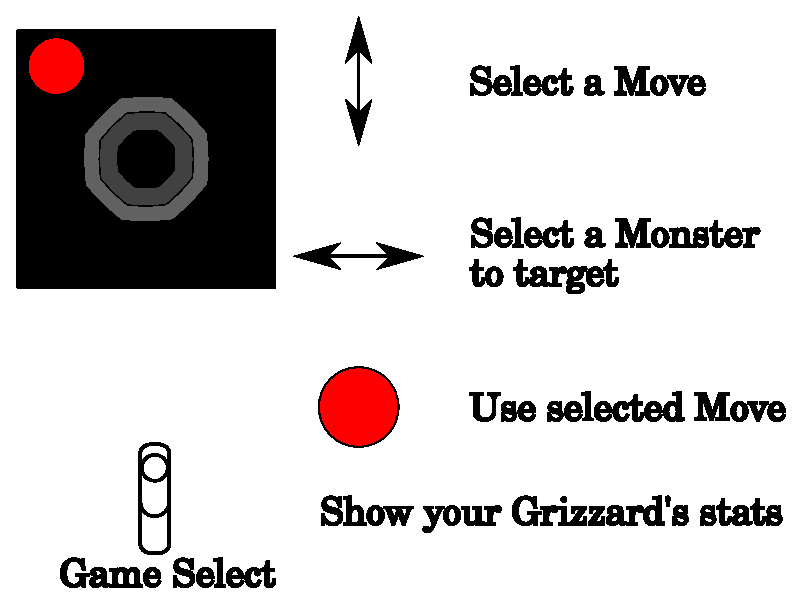
\includegraphics[width=2\columnwidth]{../Manual/CombatControls.eps}
%   \end{center}
% \end{figure*}

Monsters have  begun to plague the  world of Syrex. If  you're caught by
monsters,  your Grizzard  companion  must defend  you.  You'll see  this
Combat display.

\begin{center}
  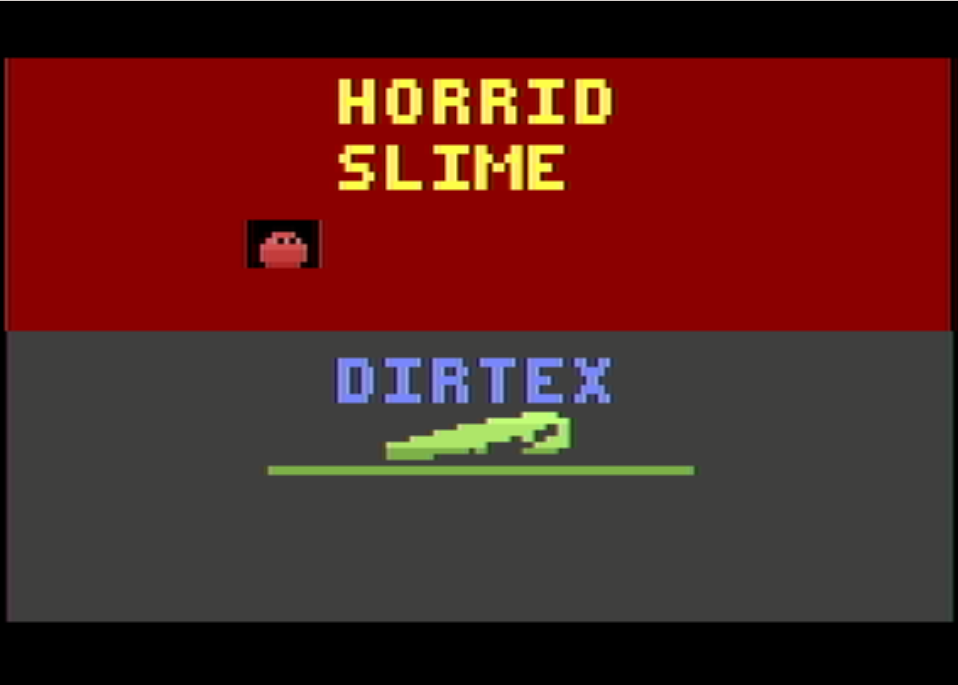
\includegraphics[width=.75\columnwidth]{../Manual/MonsterCombatNTSC.png}
\end{center}

Monsters often  travel in groups, so  you may see more  than one monster
facing you.  When it's the  monsters' turn, the  top part of  the screen
will be red (white on SECAM).

When  it's your  turn,  the  bottom part  of  the  screen, showing  your
Grizzard, will be indigo (magenta on SECAM).

The long bar beneath your Grizzard represents its hit points.

\begin{center}
  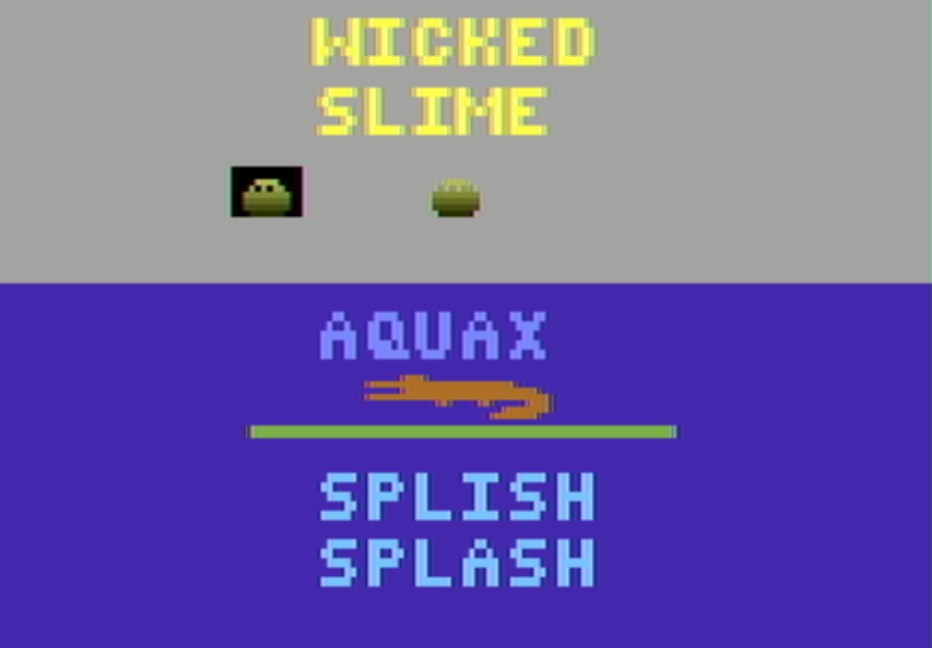
\includegraphics[width=.6667\columnwidth]{../Manual/GrizzardCombatNTSC.png}
\end{center}

Push the joystick forward and back to select a Move from those that your
Grizzard knows how to perform. Those  your Grizzard knows will appear in
light blue. If your Grizzard does \emph{not} know a Move, it will appear
in black.

To view your Grizzard's statistics, press \textbf{Game Select}.

Most Moves will target a monster. Press left or right on the joystick to
select a target. Some Moves instead affect your Grizzard itself.

When   you   have   chosen   a    Move   and   a   target,   press   the
\textbf{Fire} button.

\begin{figure*}[b]
  \begin{center}
    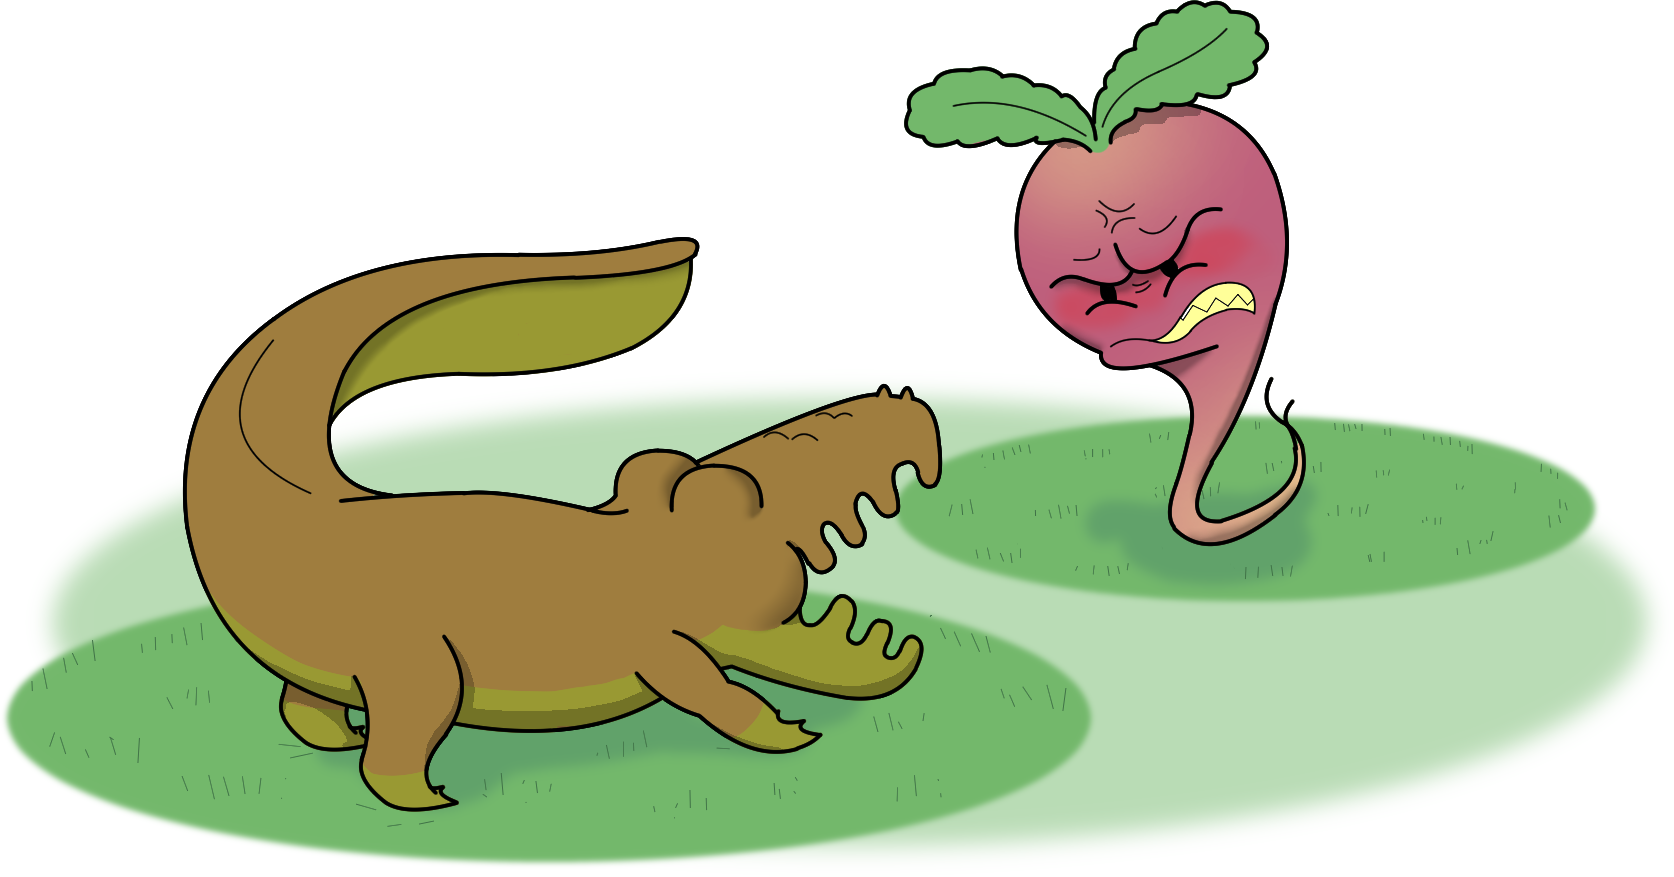
\includegraphics[width=2\columnwidth,height=\columnwidth]{../Manual/GrizzardCombat.png}
  \end{center}
\end{figure*}


\subsection{Performing a Move}

After a Move has been performed,  the creature targeted by that move may
be injured  (lose hit points)  and/or have a  Status Effect\footnote{See
  page~\pageref{sec:StatusEffects} to learn  about Status Effects} added
to  it. Status  Effects  are temporary  and last  only  the duration  of
one battle.

It's possible for a move to miss its target. If that happens, you'll see
\texttt{MISSED} appear  briefly. It's also  possible to have  a critical
success.  That move  will do  double the  usual damage,  and you'll  see
\texttt{CRIT!} appear on the screen.

If your Grizzard companion loses hit points, the bar below your Grizzard
will reduce in  length. If your Grizzard is defeated,  the monsters will
surely eat you! Your adventure will end there. \ifdefined\NOSAVE You can
resume your game from the Begin/Resume  screen, or start over. \else You
can continue from  the last Grizzard Depot you visited  by selecting the
same game slot on the Select Slot screen. \fi

If you  defeat all of  the monsters, victory  is yours! Your  score will
increase,  and you'll  return  to  the Map  screen.  You  may also  find
a potion was  left behind by the monsters. \ifdefined\DEMO  There are no
potions in the demo. \fi

% You  may choose  to run  away from  a fight,  but the  monsters will  be
% immediately healed and may still come after you.

\subsection{Grizzard Learning}

Your  Grizzard companion  may  learn from  opposing  Monsters. This  can
result in your Grizzard increasing its Attack or Defend ability, maximum
hit points, or learning a new  Move. Sometimes, your Grizzard will learn
a Move  by seeing a monster  perform it. Other times,  your Grizzard may
learn  it on  their own.  Your Grizzard  can only  learn certain  Moves.
Moves that your Grizzard does \emph{not} yet know, but is able to learn,
will appear in black.

\section{Statistics}

Press  the \textbf{Game  Select}  switch\footnote{You can  also use  the
  \encircle{C}    or     \encircle{II}    button    on     a    gamepad.
  See page~\pageref{sec:Gamepad}.} while viewing the Map, Combat screen,
or at  a Grizzard Depot  to view  your Grizzard's statistics.  Press the
\textbf{Fire} button to dismiss the Statistics screen.

At  the top  of the  Statistics screen  is a  portrait of  your Grizzard
companion, their name,  and their unique number. There  are 30 Grizzards
to catch. Can you catch them all?

\begin{center}
  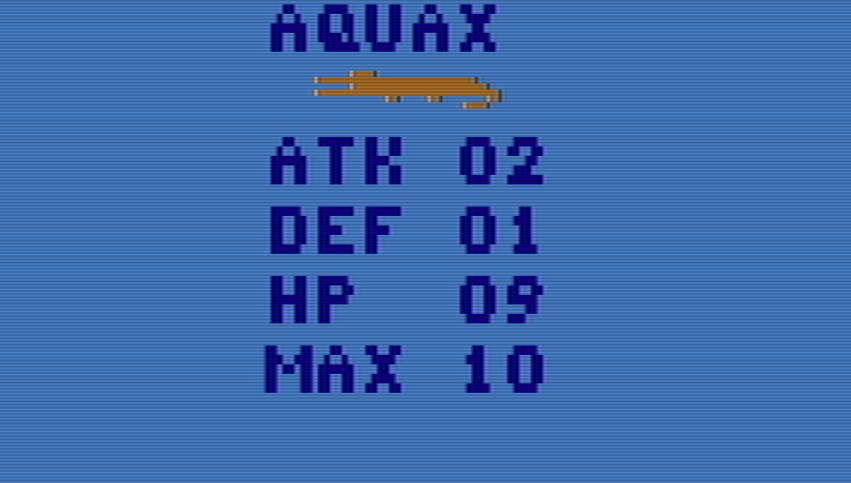
\includegraphics[width=.75\columnwidth]{../Manual/StatsScreenshotNTSC.png}
\end{center}

\begin{rdescribe}
  
\item[\texttt{ATK.}] is  the Grizzard's  \emph{Attack} ability.  This is
  the likelihood  that your Grizzard will  hit and cause damage  when it
  attacks a monster. Some Moves cause more damage than others.
  
\item[\texttt{DEF.}] is  the Grizzard's  \emph{Defend} ability.  This is
  how likely your Grizzard is to avoid being hurt by a monster's Move.

\item[\texttt{HP}]  is  the  Grizzard's  \emph{hit  points}  or  health.
  When  monsters hit  your Grizzard,  this  value will  decrease. If  it
  reaches zero, your game is over.

\item[\texttt{MAX}]  is   the  Grizzard's  \emph{maximum   hit  points}.
  Your Grizzard can only gain hit points up to this amount.
  
\end{rdescribe}

The Attack  ability, Defend  ability, or  Maximum Hit  Points may  go up
a bit after you defeat a party of monsters. Grizzards will advance their
statistics  faster  at   first,  then  more  slowly   as  they  increase
their abilities.

If you are currently in a  combat encounter, there may be Status Effects
that could change the effectiveness  of your Moves. These are \emph{not}
displayed on the Statistics screen.

\section{Status Effects}\label{sec:StatusEffects}

A Move can affect its target with Status Effects. There are six possible
Status Effects:

\begin{rdescribe}
\item[\texttt{SLEEP}] A  creature cannot  move on their turn.  There is
  a 50\% chance of waking up.
\item[\texttt{ATK UP} / \texttt{ATK DN}] Raises or lowers the creature's
  effective Attack ability.
\item[\texttt{DEF UP} / \texttt{DEF DN}] Raises or lowers the creature's
  effective Defend ability.
\item[\texttt{MUDDLE}]  A  creature will  choose  its  Moves at  random.
  There is a 50\% chance of clearing its mind.
\end{rdescribe}

These status  effects last only  the duration  of one battle.  They also
\emph{cannot} be stacked. For example: Once your attack has been raised,
it cannot be raised further.

\section{Scoring}

When you defeat a monster, you'll  earn points. The number of points you
earn will increase  as you defeat more difficult monsters.  You can also
earn points for some other actions you take in the game.

The score earned can be increased by:

\begin{ritemize}
\item \ldots{}playing  in Expert  mode (by  setting the  Left Difficulty
  Switch to the ``A'' position).
\item \ldots{}defeating the larger ``boss'' version of a monster.
\item  \ldots{}playing the  game  in  New Game  Plus  mode after  having
  defeated the final boss.
\end{ritemize}

The score for  defeating a monster will be increased  to $2\times$ for any
one of these  factors, to $3\times$ for  any two of these  factors, and to
$4\times$ if all three are true.

\section{Winning the Game}

You can  win the  game by  discovering what dark  forces are  behind the
onslaught of so many monsters, and defeating them.

You'll  be rewarded  with  a  special screen  when  you've defeated  the
final boss, showing  your name, score, and the number  of Grizzards that
have joined you.

\subsection*{New Game Plus}\label{sec:NewGamePlus}

Once  you've won  the game,  you can  keep playing!  On the  screen that
appears when you win, press \textbf{Game  Reset} on your console to save
your progress and create a ``new game, plus.''

You'll gain both  of the starting Grizzards that you  had not chosen the
first time, as well as all  your trained Grizzards. Monsters will become
more difficult — but also yield more points when defeated.


\section{Game Over}

If  you fail  in  your mission,  your  game is  over.  However, you  can
continue. You'll start over from  \ifdefined\NOSAVE the beginning of the
game, with your current progress. \else the last Grizzard Depot that you
had visited. \fi

\begin{center}
  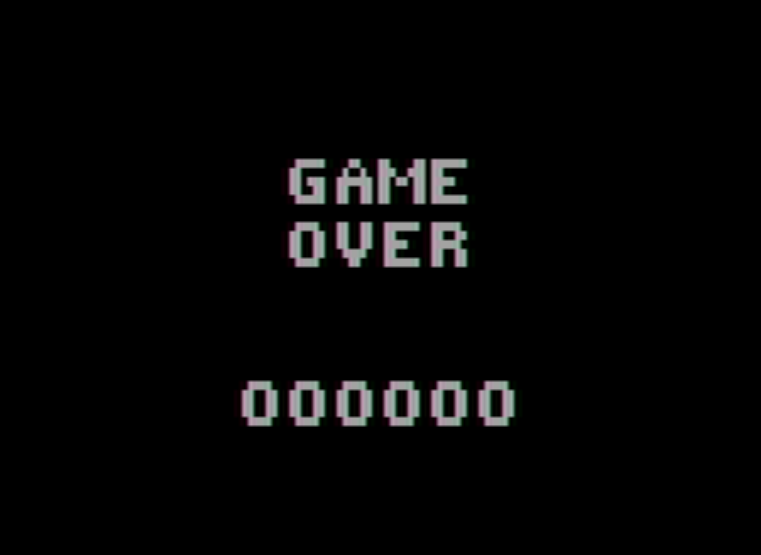
\includegraphics[width=.75\columnwidth]{../Manual/GameOverNTSC.png}
\end{center}

\section{Starting Over}\label{Starting Your Adventure Over}

\ifdefined\NOSAVE

When  you  start  the  game,  you can  \texttt{BEGIN}  a  new  game,  or
\texttt{RESUME}  your existing  game.  If  you begin  a  new game,  your
previous progress will be erased.

\else

If you want to erase your progress and start again, you must:

\begin{ritemize}
\item Go  to the Select Slot  screen, and press \textbf{Game  Select} or
  move  the joystick  left and  right until  you see  the slot  you want
  to erase.
\item Set both  of the Difficulty Switches on your  console to the ``A''
  (Advanced or Expert) position.
\item Pull  back on the  joystick, and \emph{while holding  the joystick
    back} press \emph{and hold} the \textbf{Fire} button.
\item If you're \emph{sure} you want to erase your game's progress, then
  \emph{without}  letting  go  of  the \textbf{Fire}  button,  push  the
  joystick  forward. \ifdefined\DEMO  Your  game record  will be  erased
  \emph{immediately}. \fi
\end{ritemize}

\begin{center}
  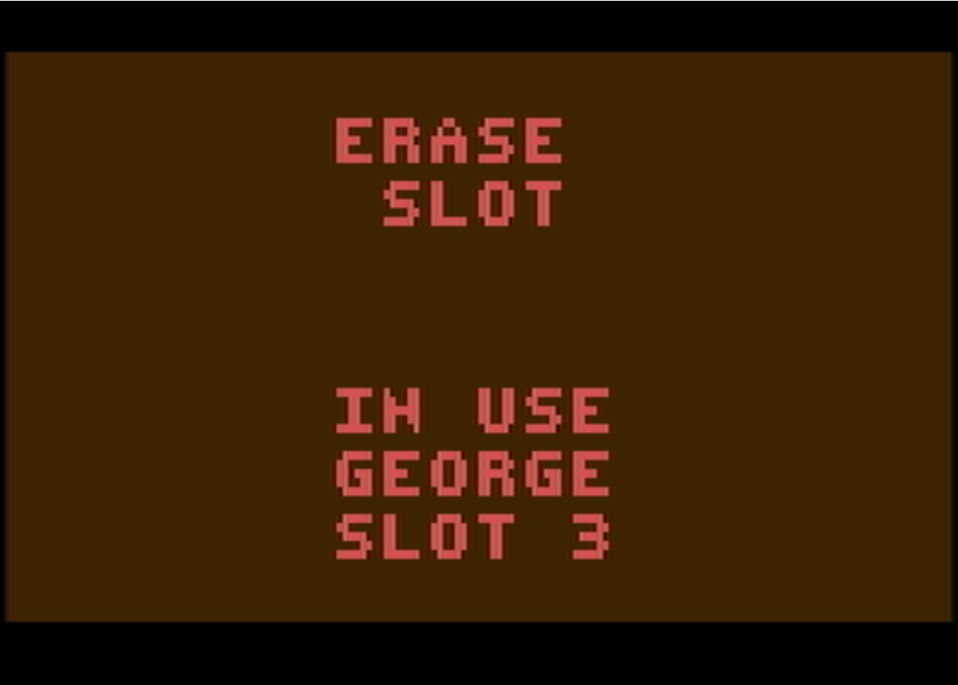
\includegraphics[width=.75\columnwidth]{../Manual/EraseSlotNTSC.png}
\end{center}

\ifdefined\DEMO

\emph{Once your game record has been  erased, you cannot recover it, so
  think carefully before you erase it.}

\else

Make sure  you want to  erase your game.  Press the joystick  forward or
back to make your choice, and press the \textbf{Fire} button.

\begin{center}
  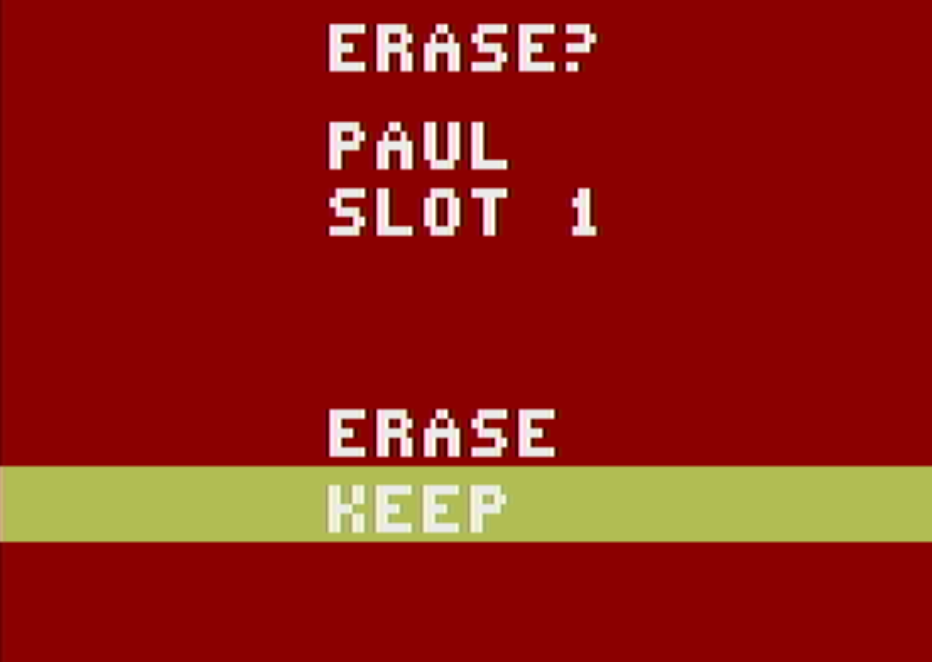
\includegraphics[width=.75\columnwidth]{../Manual/ConfirmEraseNTSC.png}
\end{center}

\fi

The Left  Difficulty Switch is also  used to increase the  difficulty of
the  game.  After  erasing  your  progress,  you  may  return  the  Left
Difficulty  Switch  to  your  desired position.  (On  SECAM,  the  Right
Difficulty Switch is used to pause the game.)

\subsection{Protecting Your Game Record}

You  cannot erase  a  game  in progress  (or  un-erase  it) unless  both
Difficulty  Switches are  in the  ``A'' (Advanced  or Expert)  position.
To protect your game from being erased, set either one of the Difficulty
Switches to the ``B'' (Beginner or Novice) position.

\ifdefined\DEMO\else

\subsection{Recovering an Erased Game}

If you have \emph{just} erased a game's progress, and no one has started
a new game using the same slot yet, you may be able to un-erase it.

To recover  an erased game,  follow the same steps  as if you  wanted to
erase  a game.  Press  left and  right  on the  joystick  to select  the
now-empty slot (the screen will say \texttt{BEGIN}). Set both Difficulty
Switches to  the ``A'' (Advanced or  Expert) position. Pull back  on the
joystick,  and \emph{while  holding the  joystick back}  press \emph{and
  hold} the \textbf{Fire} button.

If your  game's progress can be  recovered, you'll see that  the slot is
\texttt{ERASED} with your name. Press  forward on the joystick. The game
will immediately become available to resume.

It is \emph{not possible} to recover  a saved game's progress once a new
game has been started in the same memory slot. If you accidentally start
a new  game, but have  not confirmed your  name yet, \emph{turn  off the
  power briefly}, then try the preceding recovery steps.

\fi

\fi % not-nosave

\ifdefined\ATARIAGESAVE\pagebreak\fi

\chapter{Grizzards and Moves}\label{ch:Grizzards}

There are  30 Grizzards in  the game world,  each with their  own unique
starting attributes and  sets of Moves. \ifdefined\NOSAVE  In this demo,
you  can play  with only  one Grizzard  at a  time. Other  Grizzards are
available  with  a memory  device  or  the  retail cartridge.  \fi  Each
Grizzard is able to learn eight different Moves, in addition to the move
\texttt{RUN AWAY}. It's up to you  to discover which Moves each Grizzard
is able to learn.

\section{Metamorphosis}

Many Grizzards  can metamorphose into a  new form when they  have gained
a certain  amount of experience. The  new Grizzard may be  able to learn
different Moves and have improved statistics.


% When you begin your adventure, you can choose one of the following three
% Grizzards as your initial companion.

% \ifdefined\ATARIAGESAVE
% \vfill
% \fi

\ifdefined\DEMO\else

\pagebreak

\section{Dirtex}

\begin{center}
  \vspace{11pt}
  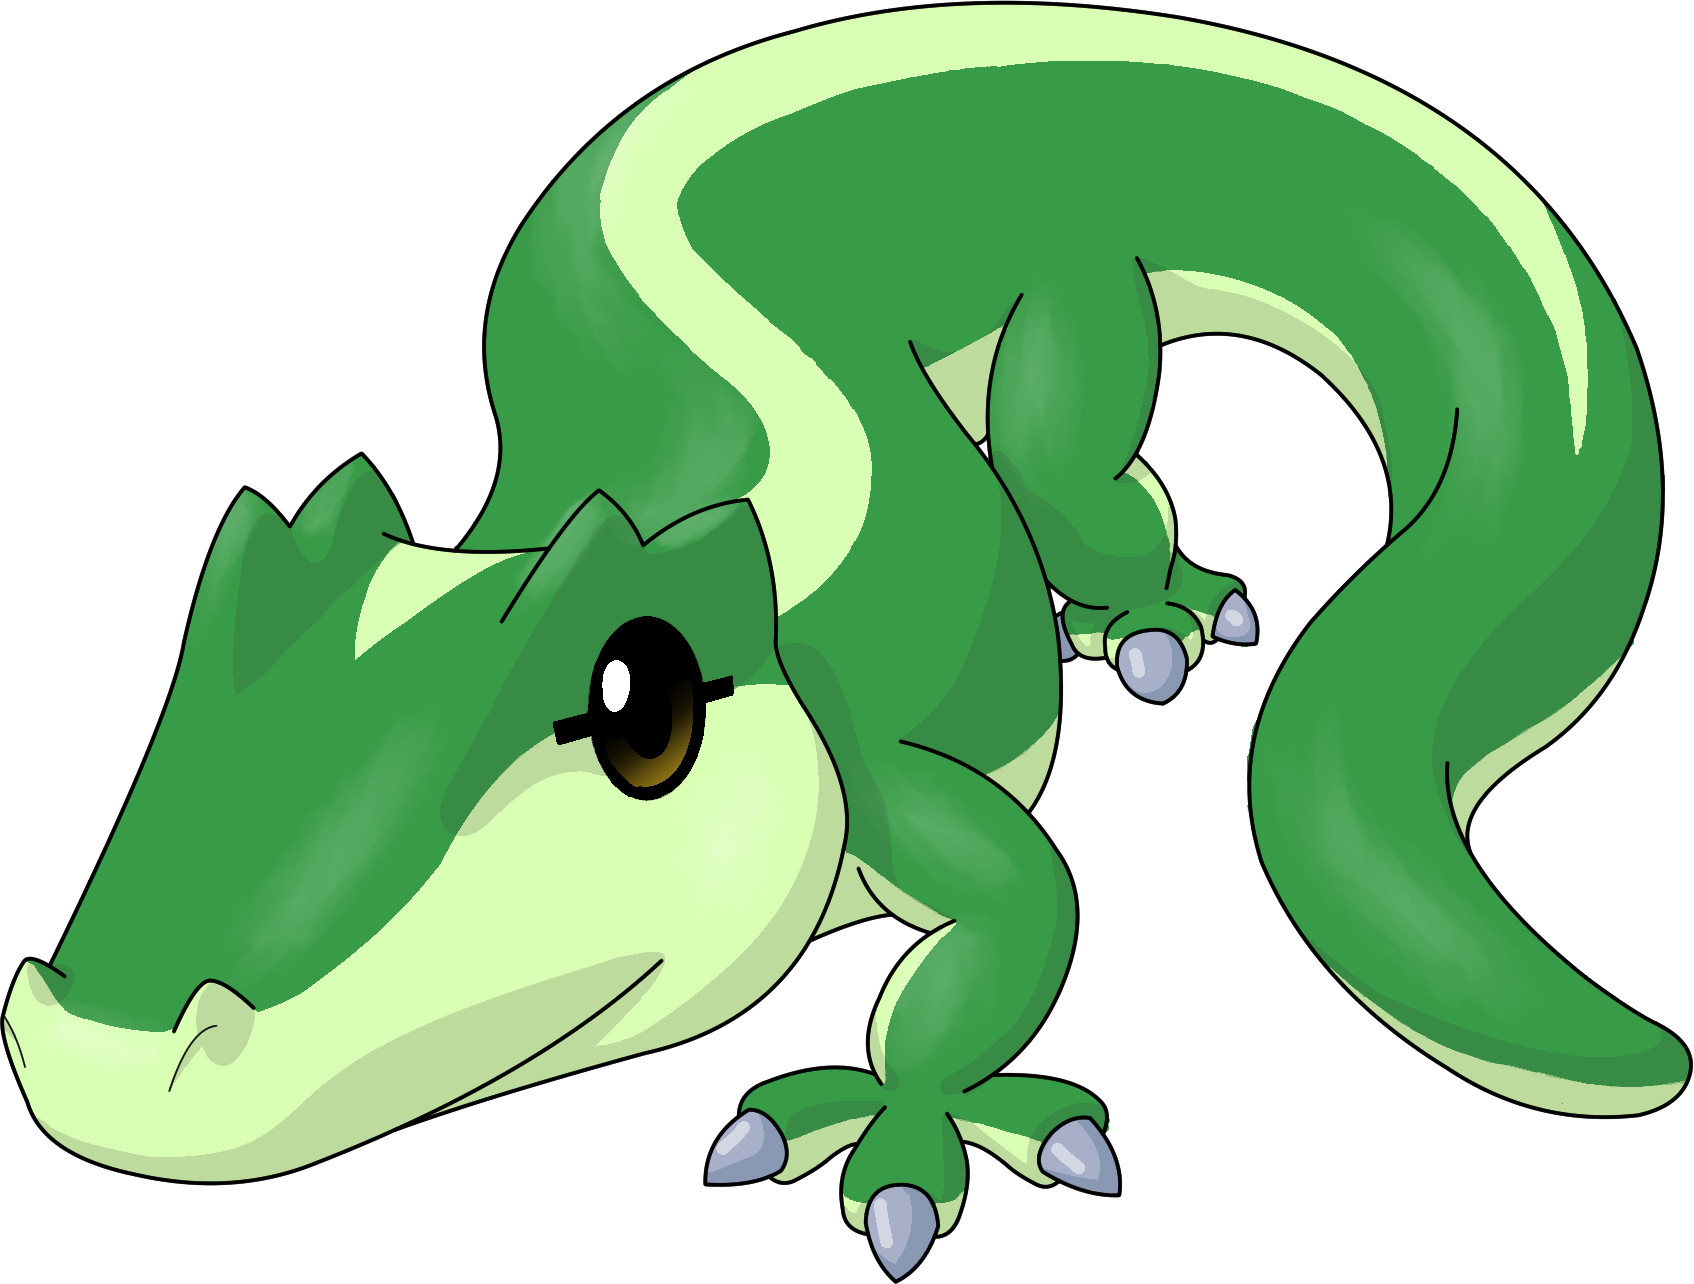
\includegraphics[width=\columnwidth]{../Manual/Dirtex.png}
\end{center}

\noindent{}The  green Grizzard  Dirtex (Num.  \texttt{01}) lives  in the
desert. It can learn these Moves:

\begin{ritemize}
\item \texttt{KICK DIRT} --- kick dirt at the enemy, causing some damage
  to them.
\item \texttt{BURY DEEP} --- try to bury the enemy, which may cause them
  to fall asleep.
\item  \texttt{DIRTY FOOT}  --- causes  some  damage and  may lower  the
  enemy's Defend ability.
\item \texttt{LOAMY FEAR} --- may lower the enemy's Attack ability.
\item \texttt{DUSTY EYES} --- may lower the enemy's Defend ability.
\end{ritemize}

When Dirtex gains enough experience, it will metamorphose into Lander.

\fi

\pagebreak

\section{Aquax}

\begin{center}
  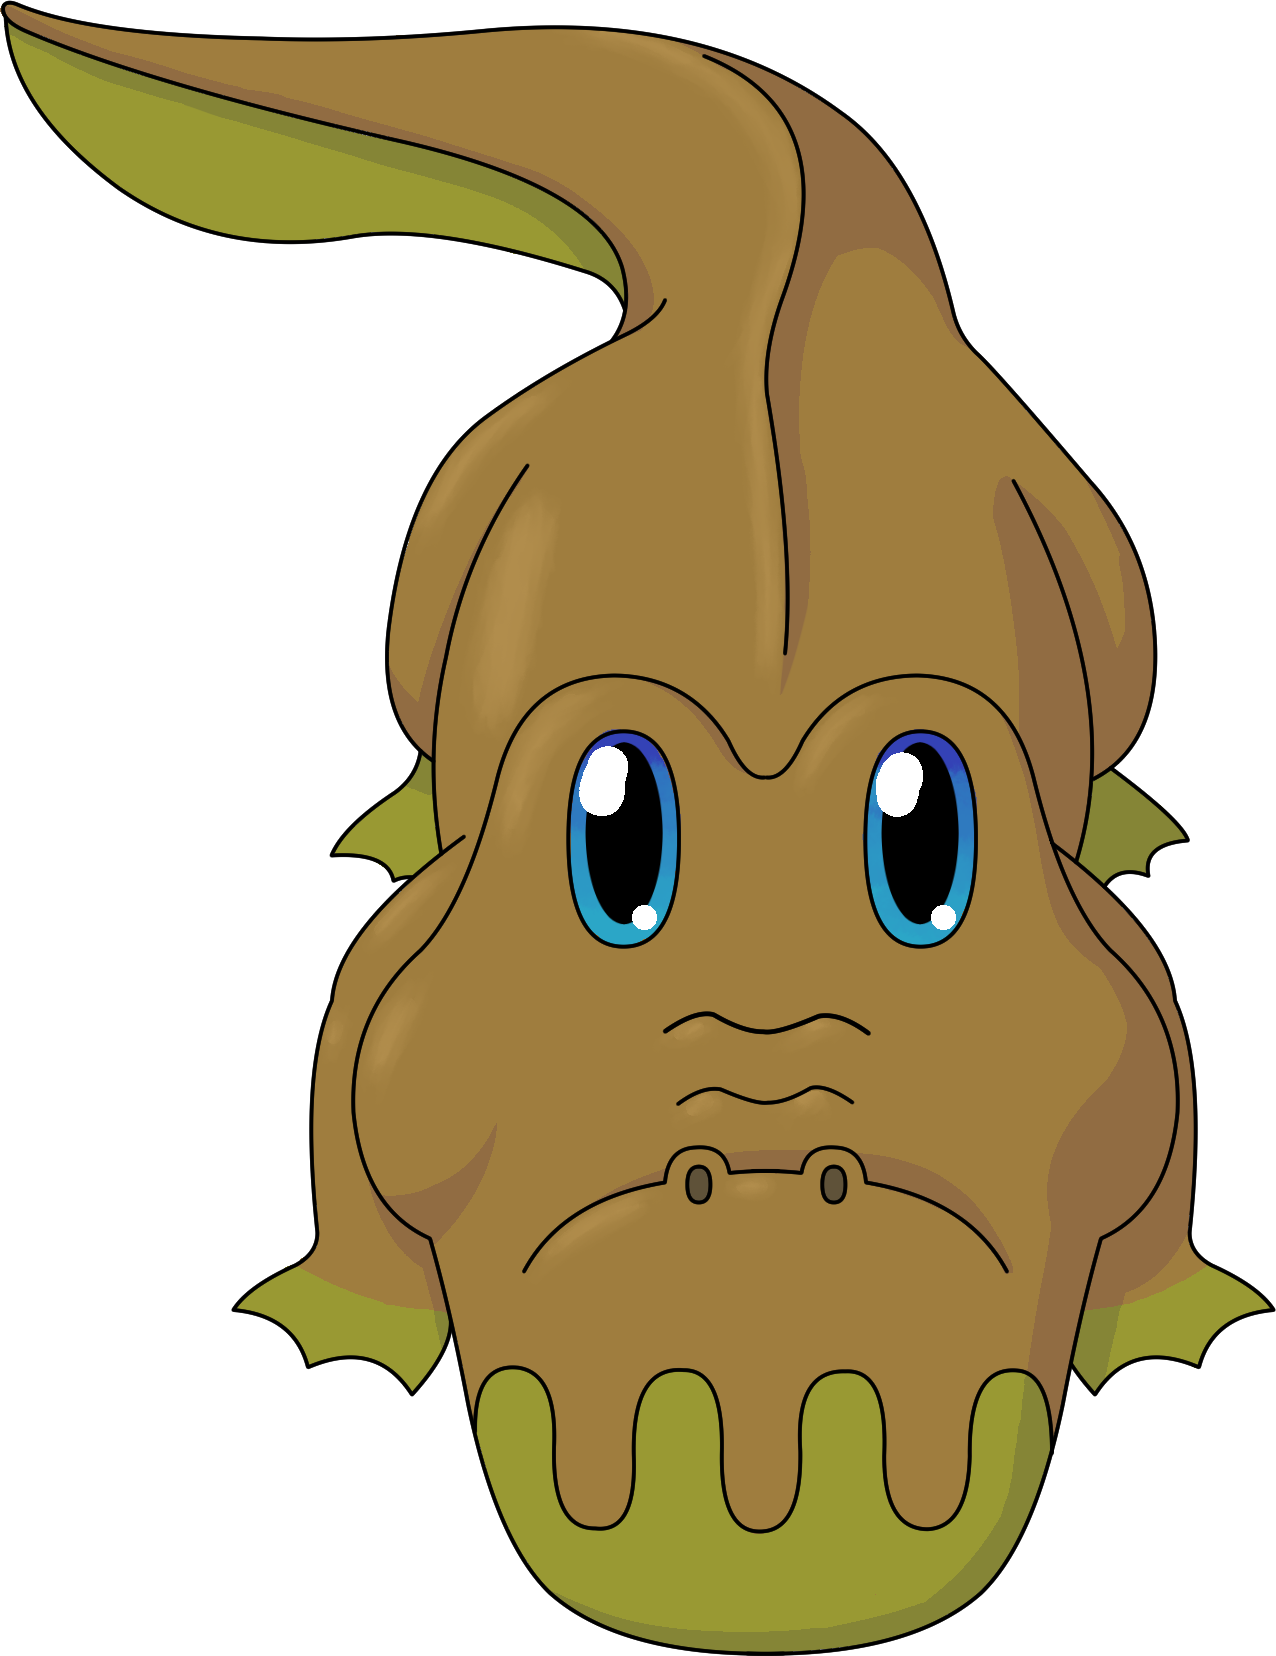
\includegraphics[width=.7\columnwidth]{../Manual/Aquax.png}
\end{center}


\noindent{}Aquax is a  brown Grizzard (Num. \texttt{02})  which lives in
the water. It can learn these Moves:

\begin{ritemize}
\item  \texttt{SPLISH SPLASH}  --- splash  water at  the enemy,  causing
  some damage. 
\item \texttt{RAISE HOPE} --- may increase its own Defend ability.
\item \texttt{SURE SPLASH} --- may increase its own Attack ability.
\item \texttt{QUICK FOOT}  --- causes some damage and  may also decrease
  the enemy's Defend ability.
\item \texttt{GREAT MOJO}  --- causes some damage and  may also decrease
  the enemy's Attack ability.
\end{ritemize}

With enough experience, Aquax can metamorphose into Sailor.

\ifdefined\DEMO\else

\pagebreak

\section{Airex}

\begin{center}
  \vspace{10pt}
  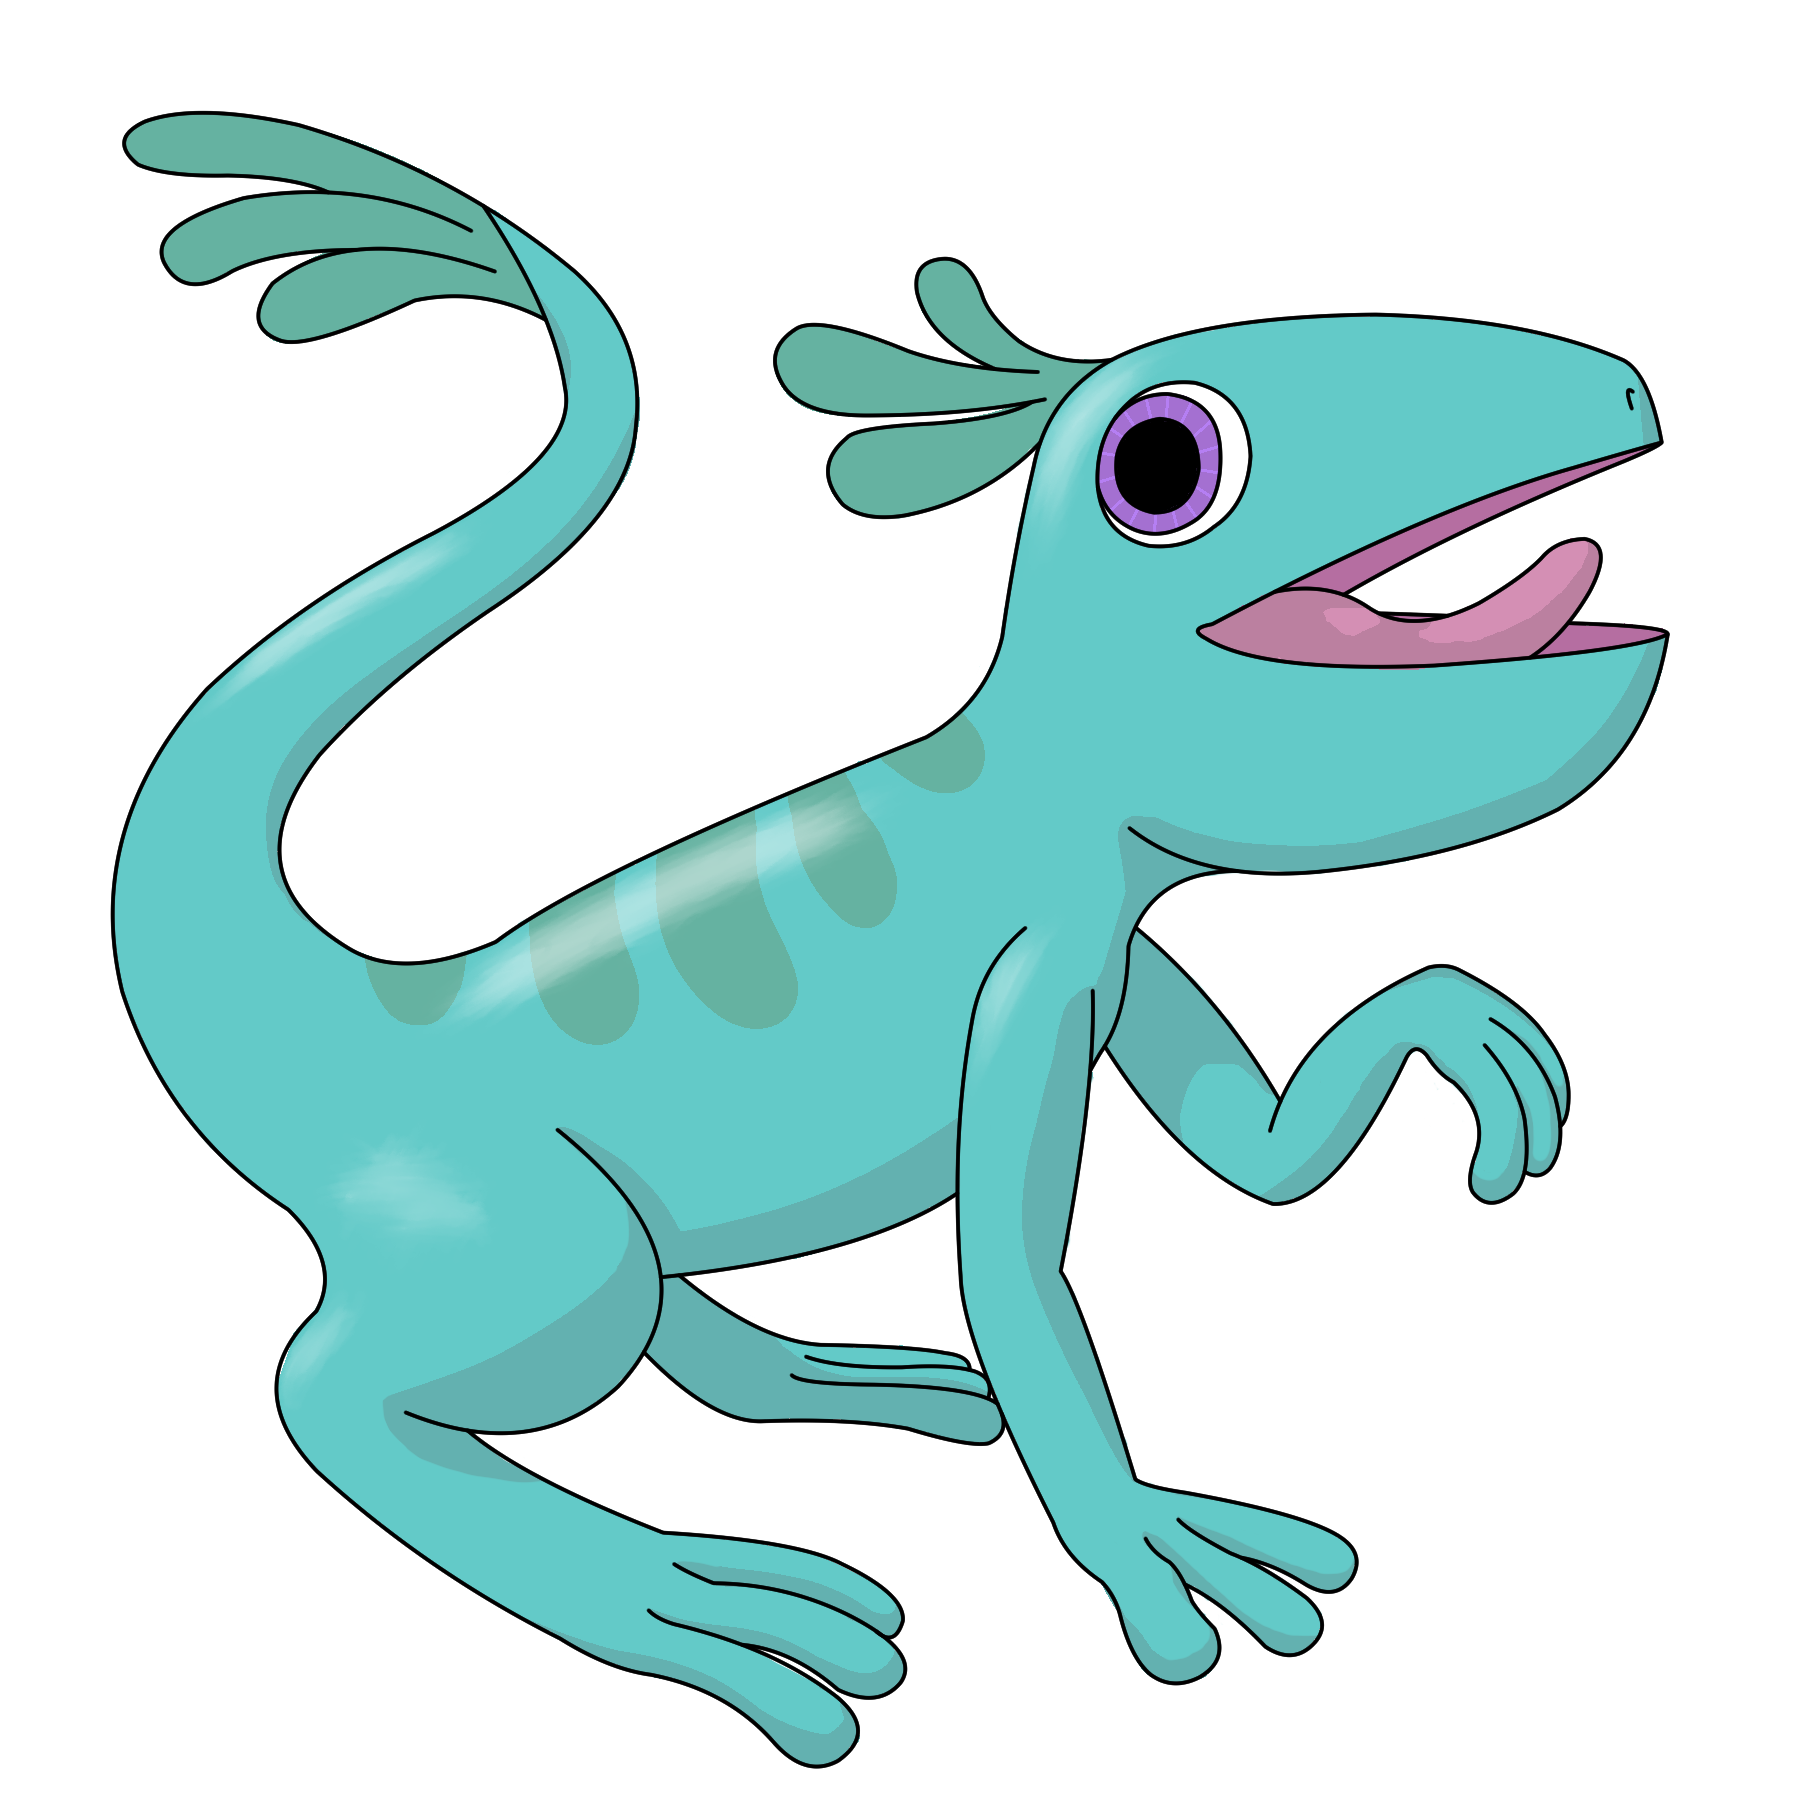
\includegraphics[width=.8\columnwidth]{../Manual/Airex.png}
\end{center}

\noindent{}Airex is  a teal Grizzard  (Num. \texttt{03}) which  lives in
the trees. It can learn these Moves:

\begin{ritemize}
\item \texttt{MILD SHOCK} --- shocks  the enemy with static electricity,
  causing some damage.
\item \texttt{WIND FIGHT} --- causes a bit more damage than \texttt{MILD SHOCK}.
\item \texttt{STEAL ATTACK} --- may lower the enemy's Attack ability.
\item \texttt{STEAL DEFEND} --- may lower the enemy's Defend ability.
\item \texttt{STEAL TURN} --- may put the enemy to sleep.
\end{ritemize}

When Airex gains enough experience, it will metamorphose into Flyer.

\fi

%% \pagebreak

\section{Healing}

Most Grizzards can learn healing Moves as well. Some examples:

\begin{ritemize}
\item \texttt{FIRST AID} --- heals a small amount of health.
\item \texttt{SIMPLE CURE} --- heals a bit larger amount of health.
\item \texttt{COMMON CURE} --- heals even more health.
\end{ritemize}

You can also heal your Grizzard  by visiting a Grizzard Depot, or giving
them a Potion. To use a  potion, press the \textbf{Fire} button while on
the Map screen. You cannot use a potion during a battle. \ifdefined\DEMO
There are no potions in this demo. \fi

\section{Running Away}

The  Move \texttt{RUN  AWAY}  lets  you try  to  escape  from a  battle.
Your  Grizzard will  \emph{not}  be  healed if  you  run  away, but  the
monsters that you were facing will be healed immediately.

Certain  monsters  are too  terrifying  to  escape. When  you  encounter
a ``boss'' monster like this, it will  be a duel to the death. Watch out
for their unique shape on the map screen.

\pagebreak

\twocolumn[\chapter{Monsters}]

A slew of monsters are arriving in Syrex, terrorizing the land.

{%%\raggedright
\englishskip

\lettrine[image=true,                lines=4,               findent=3pt,
nindent=3pt]{../Manual/Wicked-Slime.png}\nobreak\hspace{.2em plus 0}Wicked  Slimes  are
weak slime  monsters that  your Grizzard  can kill  fairly easily  … but
beware when they travel in large packs.

\englishskip

\lettrine[image=true,                lines=4,               findent=3pt,
nindent=3pt]{../Manual/Horrid-Slime.png}\nobreak\hspace{.2em plus 0}Horrid~Slimes~are
more dangerous  than a  Wicked Slime.  A Horrid  Slime may  survive your
attacks until you've learned some new Moves.

\englishskip

\lettrine[image=true,                lines=4,               findent=3pt,
nindent=3pt]{../Manual/Sky-Mutant.png}\nobreak\hspace{.2em plus 0}Sky~Mutants~roam
the~roads~north~of Mount~Peshon~looking for~civilians~to abduct.

\englishskip

\lettrine[image=true,                lines=4,               findent=3pt,
nindent=3pt]{../Manual/Round-Robin.png}\nobreak\hspace{.2em plus 0}Round   Robins   are
colorful giant birds  who live in the area of  Mount Peshon. Their beaks
and claws are dangerous.

\ifdefined\ATARIAGESAVE\pagebreak\else\englishskip\fi

\lettrine[image=true,                lines=4,               findent=3pt,
nindent=3pt]{../Manual/R.O.U.S..png}\nobreak\hspace{.2em plus 0}Rodents of Unusual Size
are one of the  dangers of the Fire Bog (but I  don't think they exist).
They're known to attack pirates and princesses alike.

\englishskip

\lettrine[image=true,                lines=4,               findent=3pt,
nindent=3pt]{../Manual/Flame-Doggo.png}\nobreak\hspace{.2em plus 0}Flame   Doggos   are
a danger of the  Fire Bogs. These beasts often roam  in packs, and their
fur is on fire.  Avoid the Fire Bogs until you have  begun to train your
Grizzard to have a higher Attack ability.

\englishskip

\lettrine[image=true,                lines=4,               findent=3pt,
nindent=3pt]{../Manual/Fire-Panda.png}\nobreak\hspace{.2em plus 0}Fire~Pandas~are~a~bit
like  red  pandas,  or  firefoxes,  and  quite  a  bit  more  dangerous.
Unlike a firefox,  these beasts actually dish out  fire-based attacks on
their victims.

\englishskip

\lettrine[image=true,                lines=4,               findent=3pt,
nindent=3pt]{../Manual/Vorpal-Bunny.png}\nobreak\hspace{.2em plus 0}Vorpal  Bunnies are
a  powerful monster  that will  take a  few hits  to kill.  Beware their
attack Moves, though! You may find Vorpal Bunnies in the Spiral Woods.

\englishskip

\lettrine[image=true,                lines=4,               findent=3pt,
nindent=3pt]{../Manual/Will-O-Wisp.png}\nobreak\hspace{.2em plus 0}Will-O-Wisps     are
bright,  floating sparks  that  are  known to  travel  in large  groups.
Once  your Attack  ability is  high  enough to  hit them,  they go  down
quickly, but they have very strong defenses!

\englishskip

\lettrine[image=true,                lines=4,               findent=3pt,
nindent=3pt]{../Manual/Cave-Bat.png}\nobreak\hspace{.2em plus 0}Cave~Bats~are sometimes~seen~in the
tunnels  beneath Mount  Peshon. They  may  swoop down  from the  ceiling
and attack!

\englishskip

\lettrine[image=true,                lines=4,               findent=3pt,
nindent=3pt]{../Manual/QuestionMark.png}\nobreak\hspace{.2em plus 0}A~Grue~is~a
sinister, lurking presence in the dark places of the earth. Its favorite
diet is adventurers, but its insatiable appetite is tempered by its fear
of light. No Grue  has ever been seen by the light of  day, and few have
survived its fearsome jaws to tell  the tale. If you're not careful, you
are likely to be eaten by a Grue.

\englishskip

\lettrine[image=true,                lines=4,               findent=3pt,
nindent=3pt]{../Manual/Venom-Sheep.png}\nobreak\hspace{.2em plus 0}Venom   Sheep   seem
like  harmless  fluffy creatures,  until  they  lash  out with  a  firey
flare --- or slap you with a wet noodle.

\ifdefined\ATARIAGESAVE\pagebreak\else\englishskip\fi

\lettrine[image=true,                lines=4,               findent=3pt,
nindent=3pt]{../Manual/Crazy-Fox.png}\nobreak\hspace{.2em plus 0}Crazy Foxes are likely
to unleash a great deal of pain. It's said that they were never actually
foxes to begin with, but were created already crazy.

\englishskip

\lettrine[image=true,                lines=4,               findent=3pt,
nindent=3pt]{../Manual/Viking-Turtle.png}\nobreak\hspace{.2em plus 0}Viking     Turtles
live  near the  Spiral  Woods.  They crawl  from  the  trees to  pillage
unsuspecting travelers, but they do move \emph{very} slowly.

\englishskip

\lettrine[image=true,                lines=4,               findent=3pt,
nindent=3pt]{../Manual/Radish-Goblin.png}\nobreak\hspace{.2em plus 0}Radish Goblins are
possessed plants that pluck themselves from the ground and attack unwary
travelers.  They  are  well  known   to  be  among  the  more  dangerous
root vegetables.

\englishskip

\lettrine[image=true,                lines=4,               findent=3pt,
nindent=3pt]{../Manual/Creepy-Spider.png}\nobreak\hspace{.2em plus 0}Creepy Spiders are
much bigger than the sort where you come from. Watch out for those giant
mandibles, they hurt!

\englishskip

\lettrine[image=true,                lines=4,               findent=3pt,
nindent=3pt]{../Manual/Metal-Mouse.png}\nobreak\hspace{.2em plus 0}Metal~Mice~are
extremely~durable,  so  it can  take  a  while  to  chip away  at  their
hit points.

} % \raggedright
% \section*{and many more...}

% There  are many  other monsters  roaming the  countryside across  Syrex.
% You'll have to discover the others on your own.

}

\ifdefined\ATARIAGESAVE\else

%% \pagebreak
\twocolumn[\chapter{Troubleshooting}]

\ifdefined\DEMO

\section*{Screen ``Jitters,'' freezes,  \ifdefined\TVPAL appears in black
  \& white,\fi or flashes blue}

These may  be signs that  a screen  (or the transition  between screens)
does not have the correct ``scan line'' count. This is a technical error
by the game's  developer (that's me!) and must be  corrected in the next
build of the game.

If you see these  effects (or if you are running in  an emulator, if you
notice that the scan line count is  not 262 (NTSC) or 312 (PAL or SECAM)
at       all       times)        please       report       them       to
\hred{mailto:support@star-hope.org}{support@star-hope.org} so  that they
can be corrected before the game is finished.

\fi

\section*{Sad Face Screen}

If you  see the Sad  Face screen,  the game is  trying to tell  you that
there is a problem.

From here, you can press the \textbf{Game Reset} switch to return to the
Title Screen.

\ifdefined\ATARIAGESAVE\else\ifdefined\NOSAVE\else

\subsection{Red Sad Face Screen: Memory Device Needed}

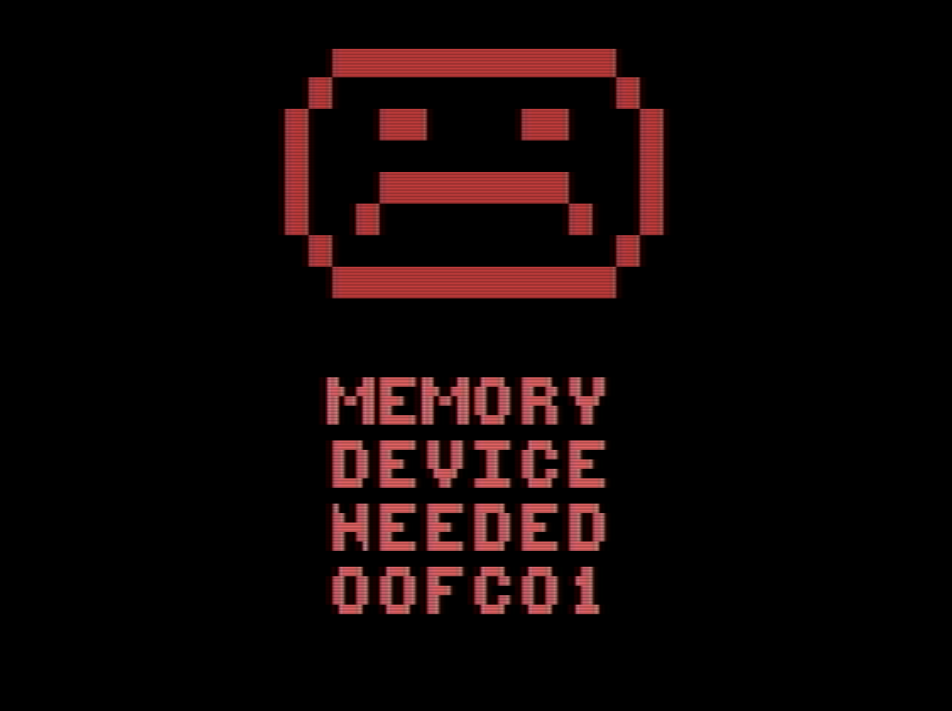
\includegraphics[width=\columnwidth]{../Manual/RedSadFaceNTSC.png}

Your  memory device  was not  found.  Connect an  AtariVox, SaveKey,  or
MemCard to the  right controller port. You should also  plug in speakers
or headphones to your AtariVox to hear game voices.

\fi\fi

\subsection{White Sad Face Screen}

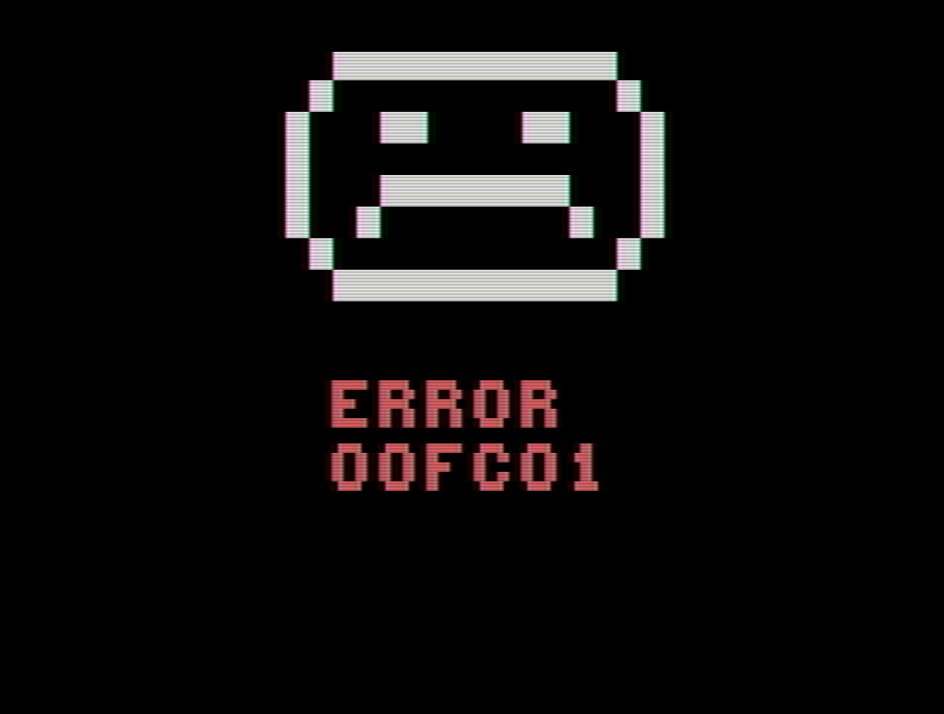
\includegraphics[width=.75\columnwidth]{../Manual/WhiteSadFaceNTSC.png}

The game  has encountered an  error and cannot continue.  Please contact
\href{mailto:support@star-hope.org}{support@star-hope.org}           for
additional assistance. Send the code  number that appears on this screen
with your email.

\ifdefined\ATARIAGESAVE\else

\section*{Pause button must be held down (7800)}

This  is believed  to  be  a side  effect  of  certain multi-carts,  eg.
PlusCart.  You  can press  \textbf{Game  Select}  instead to  view  your
Grizzard's statistics and effectively pause the game.

\section*{Joystick does not work in Stella}

Because  of  the support  for  Joy2b+  gamepads, Stella  may  (generally
wisely, but in  our case incorrectly) detect that you  would want to use
a  Keyboard  controller  rather  than   a  joystick.  In  Stella,  press
\textbf{Tab}  to access  the  settings window,  then click  \textbf{Game
  Properties}. Go  to the \textbf{Controllers}  tab in that  window, and
make sure that \textbf{Left Port} is  set to Sega Genesis (or Joystick),
and \textbf{Right  Port} is  set to  AtariVox (or  SaveKey). If  it says
Auto-Detect and  the fine  print below says  \textbf{Keyboard detected},
you will not be able to control the game.

\fi

\ifdefined\NOSAVE\else\ifdefined\ATARIAGESAVE\else

\section*{TV goes blank when entering Grizzard Depot}

Make  sure your  memory device  is  securely connected.  If your  memory
device is not connected when the game  tries to save, you may see the TV
picture remain blank while the game tries to record your progress.

\fi

\section*{No voices}

On the title  screen, you'll hear the AtariVox announce  the name of the
game. If  you don't, make  sure that the  AtariVox is connected  and the
speakers (or headphones) are connected, powered on, and turned up.

Naturally,  there are  no  voices  when playing  \ifdefined\ATARIAGESAVE
without an AtariVox device. \else with a MemCard or SaveKey device. \fi

\fi

\ifdefined\NOSAVE

%% \pagebreak
\twocolumn[\chapter{No-Save Version}]

This special  No-Save demo does not  allow you to save  your progress or
change Grizzards,  but it can be  used without a memory  device (such as
SaveKey, MemCard, or AtariVox). When you turn off power to your console,
all progress is erased.

\fi

\fi % not AtariAge release

% \ifdefined\ATARIAGESAVE\pagebreak\fi

\vfill

\pagebreak

\chapter{Credits}

\subsection{Story, Programming, Graphics}

{ Bruce-Robert Pocock }

\subsection{Music, Additional Art}

{ Zephyr Salz }

\subsection{Program Code}

The \textit{Grizzards} software includes the  VCS header file by Matthew
Dillon, Olaf ``Rhialto'' Seibert, Andrew Davie, and Peter H. Froehlich.

Binary to decimal translation is based upon code by Andrew Jacobs, based
upon code by Garth Wilson.

``Six Digit  Score'' 48 pixel  wide display  routines are based  upon an
explanation on Stella list by Erik Mooney and Bradford W. Mott.

\ifdefined\ATARIAGESAVE\else  SaveKey EEPROM  and \fi{}  AtariVox speech
synthesis driver is based upon code by Alex Herbert.

The random number generator is by AtariAge forum user \texttt{Supercat}.
Some math  functions are by AtariAge  forum user \texttt{Omega\-matrix}.
Some  math functions  were taken  from the  December 1984  \textit{Apple
  Assembly Line}.

Atari 7800  console detection logic  written by Fred Quimby  courtesy of
Darrell Spice, Jr.

\subsection{Art}

``Have  You   Played  Atari  Today''   jingle  created  by   Atari  Inc.
and transcribed by AtariAge Forum user \texttt{tigger\-the\-hun}.

AtariVox+     \ifdefined\ATARIAGESAVE\else     and     SaveKey     \fi{}
photograph\ifdefined\ATARIAGESAVE{}  is   \else{s}  are  \fi   from  the
AtariAge store.  \ifdefined\ATARIAGESAVE The AtariAge logo  and logotype
are the property of AtariAge. \fi

\subsection{Special Thanks}

Special ``save to cartridge'' circuitry designed by Fred Quimby.

Thanks to  SmittyB for helping  get the  gamepad support working  on the
Atari 7800.

Thanks to Albert Yarusso for publication support.

Special thanks  to everyone in  the Stella and AtariAge  communities for
making this game possible.

\subsection{Testers}

Philip Clark,  Dany Santana,  James Earl  O'Brien, Tanya  O'Brien, Darcy
Troy Paulin,  \texttt{Mika}, \texttt{vitoco}, David  Bowen, \texttt{Fort
  Apocalypse}, and other users from the AtariAge forum.

\ifdefined\ATARIAGESAVE\else
\vfill

 \begin{center}
  \ifdefined\ATARIAGESAVE
  
\includegraphics[width=.6667\columnwidth]{../Manual/AtariAgeHorizontalColor.eps}

  \englishskip

  \fi
  
\includegraphics[width=.333\columnwidth]{../Manual/BRP.png}
\end{center}

\fi

\ifdefined\ATARIAGESAVE
% \begin{tikzpicture}[overlay, remember picture]
%   \node[anchor=north west, xshift=-4pt, yshift=4pt] 
%   at (current page.north west)
%   {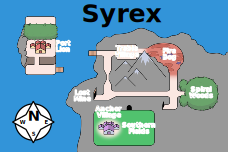
\includegraphics[width=5in,height=7in]{../Manual/SyrexMap.eps}};
% \end{tikzpicture}
\else

\clearpage
\addcontentsline{toc}{chapter}{Map of Syrex}
\thispagestyle{empty}

\begin{tikzpicture}[overlay, remember picture]
  \node[anchor=north west, xshift=-4pt, yshift=4pt] 
  at (current page.north west)
  {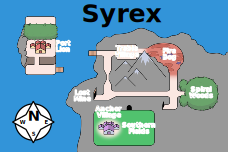
\includegraphics[width=\paperwidth,height=\paperheight]{../Manual/SyrexMap.eps}};
\end{tikzpicture}
\fi

\end{document}
